\section{Charged Particle Event Multiplicity}
\label{section: charged particle event multiplicity}

\begin{figure}[h]
	\begin{subfigure}[h]{0.32\textwidth}
%		\includegraphics[width=\textwidth]{./Chapters/multiplicity/images/reconstructed_multiplicity_2_0_4_5_measured_down.png}
		\includegraphics[width=\textwidth]{/afs/cern.ch/user/d/dvoong/cmtuser/DaVinci_v33r6/Phys/ChargedParticleMultiplicity/python/multiplicity/tracks/data_files/TrackMultiplicityPlottingJob/bk/Down/mc/-1/-1/bk/Down/mc/-1/-1/meissner_multiplicity_full/bk/Down/real/-1/-1/bk/Down/real/-1/-1/pngs/2-0_4-5_norm.png}
		\caption{$2.0 \le \eta < 4.5$}
		\label{fig: reconstructed track multiplicity measured down 2.0 - 4.5}
	\end{subfigure}
	\begin{subfigure}[h]{0.32\textwidth}
%		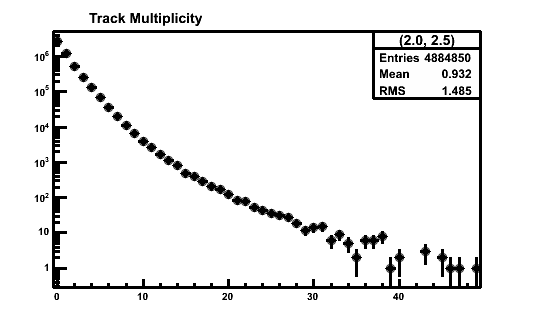
\includegraphics[width=\textwidth]{./Chapters/multiplicity/images/reconstructed_multiplicity_2_0_2_5_real_down.png}
		\includegraphics[width=\textwidth]{/afs/cern.ch/user/d/dvoong/cmtuser/DaVinci_v33r6/Phys/ChargedParticleMultiplicity/python/multiplicity/tracks/data_files/TrackMultiplicityPlottingJob/bk/Down/mc/-1/-1/bk/Down/mc/-1/-1/meissner_multiplicity/bk/Down/real/-1/-1/bk/Down/real/-1/-1/pngs/2-0_2-5_norm.png}
		\caption{$2.0 \le \eta < 2.5$}
		\label{fig: reconstructed track multiplicity measured down 2.0 - 2.5}
	\end{subfigure}
	\begin{subfigure}[h]{0.32\textwidth}
%		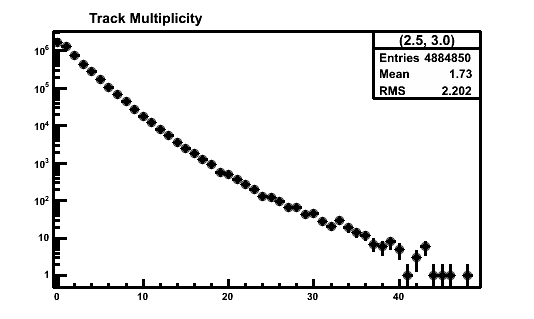
\includegraphics[width=\textwidth]{./Chapters/multiplicity/images/reconstructed_multiplicity_2_5_3_0_real_down.png}
		\includegraphics[width=\textwidth]{/afs/cern.ch/user/d/dvoong/cmtuser/DaVinci_v33r6/Phys/ChargedParticleMultiplicity/python/multiplicity/tracks/data_files/TrackMultiplicityPlottingJob/bk/Down/mc/-1/-1/bk/Down/mc/-1/-1/meissner_multiplicity/bk/Down/real/-1/-1/bk/Down/real/-1/-1/pngs/2-5_3-0_norm.png}
		\caption{$2.5 \le \eta < 3.0$}
		\label{fig: reconstructed track multiplicity measured down 2.5 - 3.0}
	\end{subfigure}
	\begin{subfigure}[h]{0.32\textwidth}
%		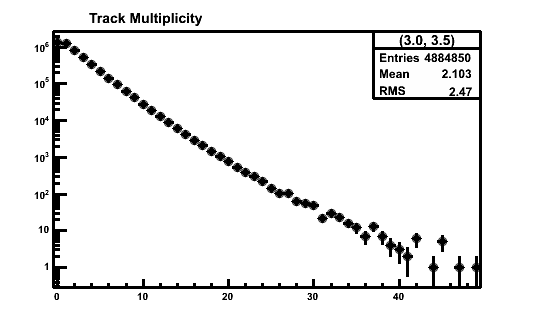
\includegraphics[width=\textwidth]{./Chapters/multiplicity/images/reconstructed_multiplicity_3_0_3_5_real_down.png}
		\includegraphics[width=\textwidth]{/afs/cern.ch/user/d/dvoong/cmtuser/DaVinci_v33r6/Phys/ChargedParticleMultiplicity/python/multiplicity/tracks/data_files/TrackMultiplicityPlottingJob/bk/Down/mc/-1/-1/bk/Down/mc/-1/-1/meissner_multiplicity/bk/Down/real/-1/-1/bk/Down/real/-1/-1/pngs/3-0_3-5_norm.png}
		\caption{$3.0 \le \eta < 3.5$}
		\label{fig: reconstructed track multiplicity measured down 3.0 - 3.5}
	\end{subfigure}
	\begin{subfigure}[h]{0.32\textwidth}
%		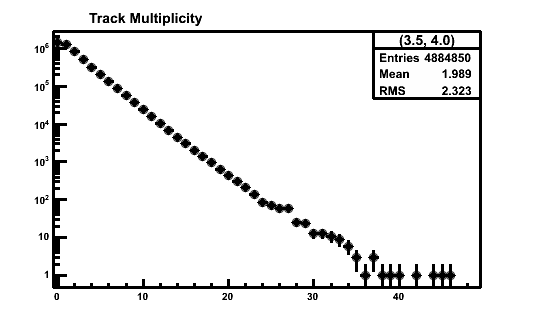
\includegraphics[width=\textwidth]{./Chapters/multiplicity/images/reconstructed_multiplicity_3_5_4_0_real_down.png}
		\includegraphics[width=\textwidth]{/afs/cern.ch/user/d/dvoong/cmtuser/DaVinci_v33r6/Phys/ChargedParticleMultiplicity/python/multiplicity/tracks/data_files/TrackMultiplicityPlottingJob/bk/Down/mc/-1/-1/bk/Down/mc/-1/-1/meissner_multiplicity/bk/Down/real/-1/-1/bk/Down/real/-1/-1/pngs/3-5_4-0_norm.png}
		\caption{$3.5 \le \eta < 4.0$}
		\label{fig: reconstructed track multiplicity measured down 3.5 - 4.0}
	\end{subfigure}
	\begin{subfigure}[h]{0.32\textwidth}
%		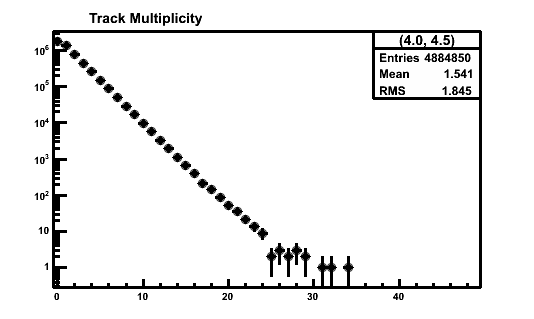
\includegraphics[width=\textwidth]{./Chapters/multiplicity/images/reconstructed_multiplicity_4_0_4_5_real_down.png}
		\includegraphics[width=\textwidth]{/afs/cern.ch/user/d/dvoong/cmtuser/DaVinci_v33r6/Phys/ChargedParticleMultiplicity/python/multiplicity/tracks/data_files/TrackMultiplicityPlottingJob/bk/Down/mc/-1/-1/bk/Down/mc/-1/-1/meissner_multiplicity/bk/Down/real/-1/-1/bk/Down/real/-1/-1/pngs/4-0_4-5_norm.png}
		\caption{$4.0 \le \eta < 4.5$}
		\label{fig: reconstructed track multiplicity measured down 4.0 - 4.5}
	\end{subfigure}
	\caption{Reconstructed track multiplicity of measured data}
	\label{fig: reconstructed track multiplicity measured}
\end{figure}

The event multiplicity distribution describes the number of tracks or charged particles produced per proton-proton interaction. The process of particle production in high energy collisions is very sensitive to phenomenological models used by MC event generators. As with the case of the charged particle densities, a series of corrections are applied to the measured track distributions to correct for detector effects such as background contributions, reconstruction efficiencies and pile-up. The charged particle densities the distributions were plotted as a function of the continuous quantities, pseudorapidity and transverse momentum. The event multiplicity distribution is plotted as a function of the discrete quantity, $N_\mathrm{ch}$, the number of charged particles or tracks in the event. In order to correct the distribution, different methods of applying the corrections are employed, these are discussed in the following sections.

\begin{figure}[h]
	\begin{subfigure}[h]{0.32\textwidth}
%		\includegraphics[width=\textwidth]{/afs/cern.ch/work/d/dvoong/private/cmtuser/DaVinci_v33r6/Phys/ChargedParticleMultiplicity/python/multiplicity/tracks/data_files/manual/plots/2_0-4_5_real_mc_comparison.png}
		\includegraphics[width=\textwidth]{/afs/cern.ch/user/d/dvoong/cmtuser/DaVinci_v33r6/Phys/ChargedParticleMultiplicity/python/multiplicity/tracks/data_files/TrackMultiplicityPlottingJob/bk/Down/mc/-1/-1/bk/Down/mc/-1/-1/meissner_multiplicity_full/bk/Down/real/-1/-1/bk/Down/real/-1/-1/pngs/comparison/2-0_4-5_comparison.png}
		\caption{$2.0 \le \eta < 4.5$}
		\label{fig: reconstructed track multiplicity measured data-mc comparison 2.0 - 4.5}
	\end{subfigure}
	\begin{subfigure}[h]{0.32\textwidth}
%		\includegraphics[width=\textwidth]{/afs/cern.ch/work/d/dvoong/private/cmtuser/DaVinci_v33r6/Phys/ChargedParticleMultiplicity/python/multiplicity/tracks/data_files/manual/plots/2_0-2_5_real_mc_comparison.png}
		\includegraphics[width=\textwidth]{/afs/cern.ch/user/d/dvoong/cmtuser/DaVinci_v33r6/Phys/ChargedParticleMultiplicity/python/multiplicity/tracks/data_files/TrackMultiplicityPlottingJob/bk/Down/mc/-1/-1/bk/Down/mc/-1/-1/meissner_multiplicity/bk/Down/real/-1/-1/bk/Down/real/-1/-1/pngs/comparison/2-0_2-5_comparison.png}
		\caption{$2.0 \le \eta < 2.5$}
		\label{fig: reconstructed track multiplicity measured data-mc comparison 2.0 - 2.5}
	\end{subfigure}
	\begin{subfigure}[h]{0.32\textwidth}
%		\includegraphics[width=\textwidth]{/afs/cern.ch/work/d/dvoong/private/cmtuser/DaVinci_v33r6/Phys/ChargedParticleMultiplicity/python/multiplicity/tracks/data_files/manual/plots/2_5-3_0_real_mc_comparison.png}
		\includegraphics[width=\textwidth]{/afs/cern.ch/user/d/dvoong/cmtuser/DaVinci_v33r6/Phys/ChargedParticleMultiplicity/python/multiplicity/tracks/data_files/TrackMultiplicityPlottingJob/bk/Down/mc/-1/-1/bk/Down/mc/-1/-1/meissner_multiplicity/bk/Down/real/-1/-1/bk/Down/real/-1/-1/pngs/comparison/2-5_3-0_comparison.png}
		\caption{$2.5 \le \eta < 3.0$}
		\label{fig: reconstructed track multiplicity measured data-mc comparison 2.5 - 3.0}
	\end{subfigure}
	\begin{subfigure}[h]{0.32\textwidth}
%		\includegraphics[width=\textwidth]{/afs/cern.ch/work/d/dvoong/private/cmtuser/DaVinci_v33r6/Phys/ChargedParticleMultiplicity/python/multiplicity/tracks/data_files/manual/plots/3_0-3_5_real_mc_comparison.png}
		\includegraphics[width=\textwidth]{/afs/cern.ch/user/d/dvoong/cmtuser/DaVinci_v33r6/Phys/ChargedParticleMultiplicity/python/multiplicity/tracks/data_files/TrackMultiplicityPlottingJob/bk/Down/mc/-1/-1/bk/Down/mc/-1/-1/meissner_multiplicity/bk/Down/real/-1/-1/bk/Down/real/-1/-1/pngs/comparison/3-0_3-5_comparison.png}
		\caption{$3.0 \le \eta < 3.5$}
		\label{fig: reconstructed track multiplicity measured data-mc comparison 3.0 - 3.5}
	\end{subfigure}
	\begin{subfigure}[h]{0.32\textwidth}
%		\includegraphics[width=\textwidth]{/afs/cern.ch/work/d/dvoong/private/cmtuser/DaVinci_v33r6/Phys/ChargedParticleMultiplicity/python/multiplicity/tracks/data_files/manual/plots/3_5-4_0_real_mc_comparison.png}
		\includegraphics[width=\textwidth]{/afs/cern.ch/user/d/dvoong/cmtuser/DaVinci_v33r6/Phys/ChargedParticleMultiplicity/python/multiplicity/tracks/data_files/TrackMultiplicityPlottingJob/bk/Down/mc/-1/-1/bk/Down/mc/-1/-1/meissner_multiplicity/bk/Down/real/-1/-1/bk/Down/real/-1/-1/pngs/comparison/3-5_4-0_comparison.png}
		\caption{$3.5 \le \eta < 4.0$}
		\label{fig: reconstructed track multiplicity measured data-mc comparison 3.5 - 4.0}
	\end{subfigure}
	\begin{subfigure}[h]{0.32\textwidth}
%		\includegraphics[width=\textwidth]{/afs/cern.ch/work/d/dvoong/private/cmtuser/DaVinci_v33r6/Phys/ChargedParticleMultiplicity/python/multiplicity/tracks/data_files/manual/plots/4_0-4_5_real_mc_comparison.png}
		\includegraphics[width=\textwidth]{/afs/cern.ch/user/d/dvoong/cmtuser/DaVinci_v33r6/Phys/ChargedParticleMultiplicity/python/multiplicity/tracks/data_files/TrackMultiplicityPlottingJob/bk/Down/mc/-1/-1/bk/Down/mc/-1/-1/meissner_multiplicity/bk/Down/real/-1/-1/bk/Down/real/-1/-1/pngs/comparison/4-0_4-5_comparison.png}
		\caption{$4.0 \le \eta < 4.5$}
		\label{fig: reconstructed track multiplicity measured data-mc comparison 4.0 - 4.5}
	\end{subfigure}
	\caption{Comparison of reconstructed track multiplicities in measured and MC simulated data}
	\label{fig: reconstructed track multiplicity measured data mc comparison}
\end{figure}

The uncorrected track multiplicities are shown in figure \ref{fig: reconstructed track multiplicity measured}. A comparison between measured and MC data is shown in figure \ref{fig: reconstructed track multiplicity measured data mc comparison}; these data shows a systematic increase in the track multiplicity in measured data, this is partly due to pile-up (which is not included in the MC simulated data) and the physics of the MC generator. Lastly a comparison between the uncorrected track multiplicity and the true particle multiplicity in MC data is shown in figure \ref{fig: reconstructed track multiplicity mc down}; this shows that the detector response varies significantly over the pseudorapidity range of the experiment with efficiency effects being more predominant at the boundaries, $2.0 \le \eta \le 2.5$ and $4.0 \le \eta \le 4.5$, and background effects being more predominant in the middle region $3.0 \le \eta \le 4.0$. 

%\ref{fig: reconstructed track multiplicity measured down}

\begin{figure}[h]
	\begin{subfigure}[h]{0.32\textwidth}
		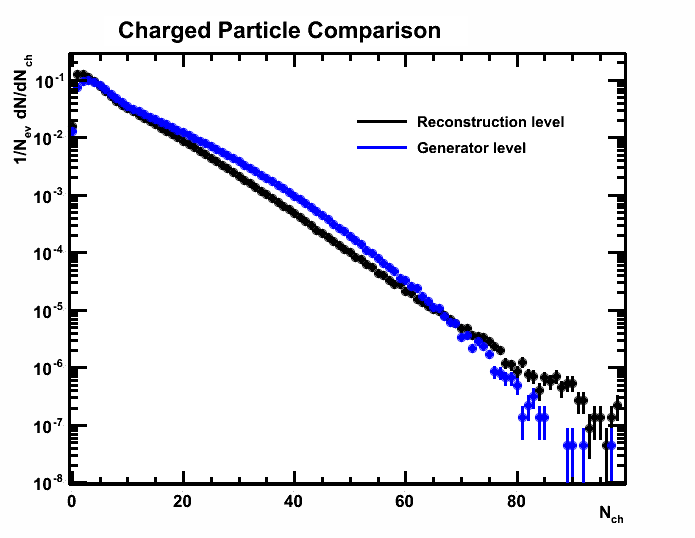
\includegraphics[width=\textwidth]{./Chapters/multiplicity/charged_particle_event_multiplicity/images/reco_gen_comparison/2_0-4_5.png}
		\caption{$2.0 \le \eta < 4.5$}
		\label{fig: reconstructed track multiplicity measured down 2.0 - 4.5}
	\end{subfigure}
	\begin{subfigure}[h]{0.32\textwidth}
		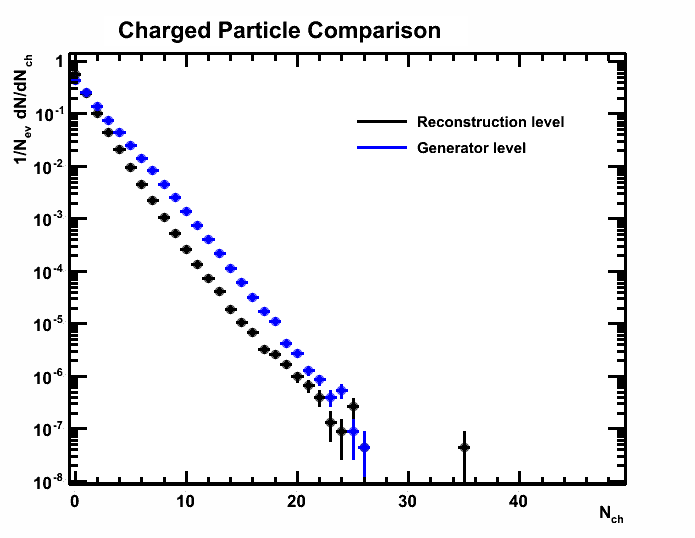
\includegraphics[width=\textwidth]{./Chapters/multiplicity/charged_particle_event_multiplicity/images/reco_gen_comparison/2_0-2_5.png}
		\caption{$2.0 \le \eta < 2.5$}
		\label{fig: reconstructed track multiplicity mc down 2.0 - 2.5}
	\end{subfigure}
	\begin{subfigure}[h]{0.32\textwidth}
		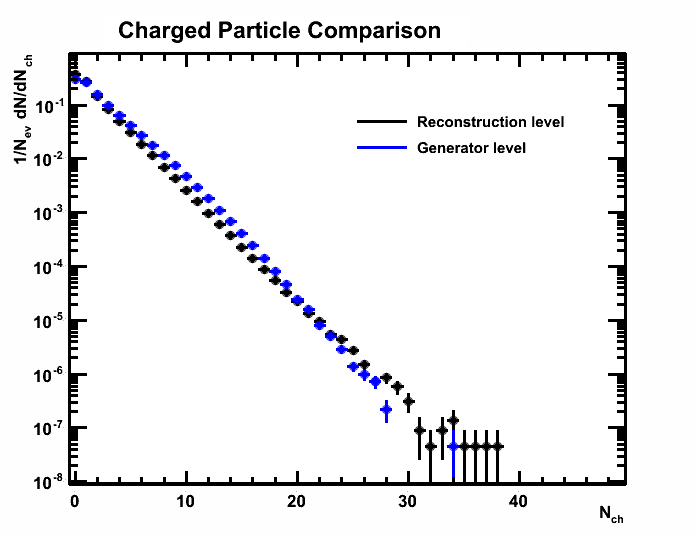
\includegraphics[width=\textwidth]{./Chapters/multiplicity/charged_particle_event_multiplicity/images/reco_gen_comparison/2_5-3_0.png}
		\caption{$2.5 \le \eta < 3.0$}
		\label{fig: reconstructed track multiplicity mc down 2.5 - 3.0}
	\end{subfigure}
	\begin{subfigure}[h]{0.32\textwidth}
		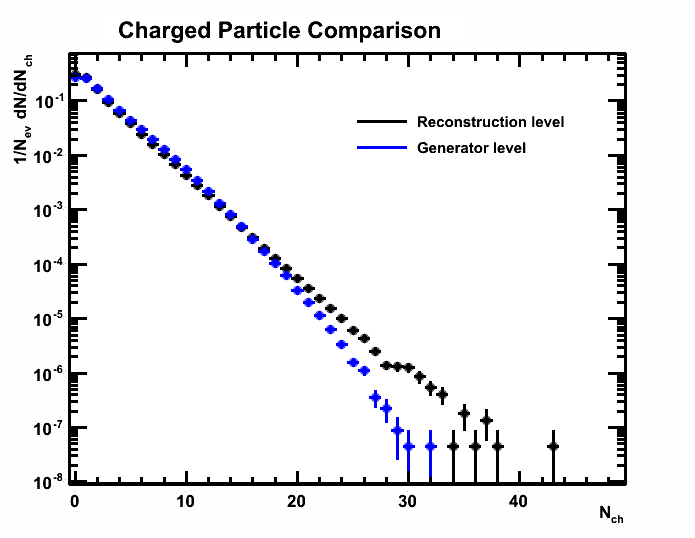
\includegraphics[width=\textwidth]{./Chapters/multiplicity/charged_particle_event_multiplicity/images/reco_gen_comparison/3_0-3_5.png}
		\caption{$3.0 \le \eta < 3.5$}
		\label{fig: reconstructed track multiplicity mc down 3.0 - 3.5}
	\end{subfigure}
	\begin{subfigure}[h]{0.32\textwidth}
		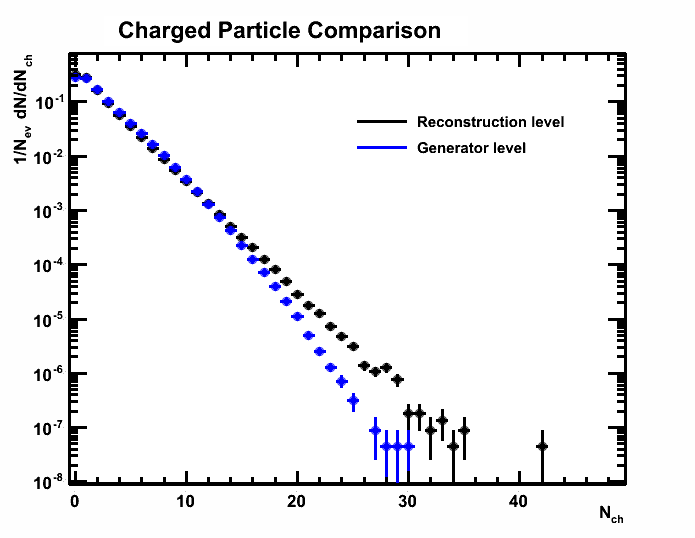
\includegraphics[width=\textwidth]{./Chapters/multiplicity/charged_particle_event_multiplicity/images/reco_gen_comparison/3_5-4_0.png}
		\caption{$3.5 \le \eta < 4.0$}
		\label{fig: reconstructed track multiplicity mc down 3.5 - 4.0}
	\end{subfigure}
	\begin{subfigure}[h]{0.32\textwidth}
		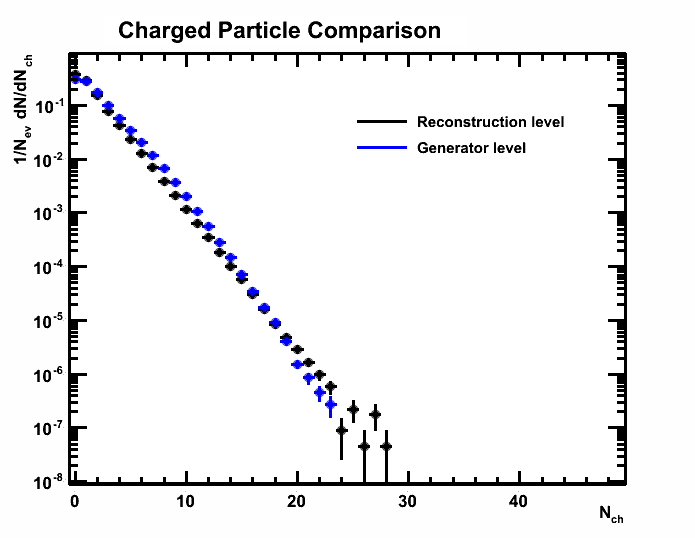
\includegraphics[width=\textwidth]{./Chapters/multiplicity/charged_particle_event_multiplicity/images/reco_gen_comparison/4_0-4_5.png}
		\caption{$4.0 \le \eta < 4.5$}
		\label{fig: reconstructed track multiplicity mc down 4.0 - 4.5}
	\end{subfigure}
	\caption{Comparison between reconstructed track multiplicities and generator charged particle multiplicities in MC simulated data.}
	\label{fig: reconstructed track multiplicity mc down}
\end{figure}


\subsection{Background Correction}
\label{subsection: charged particle multiplicity, background correction}

%\begin{figure}[h]
%	\centering
%	\begin{subfigure}{0.32\textwidth}
%		\includegraphics[width=\textwidth]{/afs/cern.ch/user/d/dvoong/cmtuser/DaVinci_v33r6/Phys/ChargedParticleMultiplicity/python/multiplicity/tracks/data_files/TrackMultiplicityPlottingJob/bk/Down/mc/-1/-1/bk/Down/mc/-1/-1/meissner_multiplicity_full/bk/Down/real/-1/-1/bk/Down/real/-1/-1/pngs/background_corrected/2-0_4-5_norm.png}
%		\caption{$2.0 \le \eta \le 4.5$}
%	\end{subfigure}
%	\begin{subfigure}{0.32\textwidth}
%		\includegraphics[width=\textwidth]{/afs/cern.ch/user/d/dvoong/cmtuser/DaVinci_v33r6/Phys/ChargedParticleMultiplicity/python/multiplicity/tracks/data_files/TrackMultiplicityPlottingJob/bk/Down/mc/-1/-1/bk/Down/mc/-1/-1/meissner_multiplicity/bk/Down/real/-1/-1/bk/Down/real/-1/-1/pngs/background_corrected/2-0_2-5_norm.png}
%		\caption{$2.0 \le \eta \le 2.5$}
%	\end{subfigure}
%	\begin{subfigure}{0.32\textwidth}
%		\includegraphics[width=\textwidth]{/afs/cern.ch/user/d/dvoong/cmtuser/DaVinci_v33r6/Phys/ChargedParticleMultiplicity/python/multiplicity/tracks/data_files/TrackMultiplicityPlottingJob/bk/Down/mc/-1/-1/bk/Down/mc/-1/-1/meissner_multiplicity/bk/Down/real/-1/-1/bk/Down/real/-1/-1/pngs/background_corrected/2-5_3-0_norm.png}
%		\caption{$2.5 \le \eta \le 3.0$}
%	\end{subfigure}
%	\begin{subfigure}{0.32\textwidth}
%		\includegraphics[width=\textwidth]{/afs/cern.ch/user/d/dvoong/cmtuser/DaVinci_v33r6/Phys/ChargedParticleMultiplicity/python/multiplicity/tracks/data_files/TrackMultiplicityPlottingJob/bk/Down/mc/-1/-1/bk/Down/mc/-1/-1/meissner_multiplicity/bk/Down/real/-1/-1/bk/Down/real/-1/-1/pngs/background_corrected/3-0_3-5_norm.png}
%		\caption{$3.0 \le \eta \le 3.5$}
%	\end{subfigure}
%	\begin{subfigure}{0.32\textwidth}
%		\includegraphics[width=\textwidth]{/afs/cern.ch/user/d/dvoong/cmtuser/DaVinci_v33r6/Phys/ChargedParticleMultiplicity/python/multiplicity/tracks/data_files/TrackMultiplicityPlottingJob/bk/Down/mc/-1/-1/bk/Down/mc/-1/-1/meissner_multiplicity/bk/Down/real/-1/-1/bk/Down/real/-1/-1/pngs/background_corrected/3-5_4-0_norm.png}
%		\caption{$3.5 \le \eta \le 4.0$}
%	\end{subfigure}
%	\begin{subfigure}{0.32\textwidth}
%		\includegraphics[width=\textwidth]{/afs/cern.ch/user/d/dvoong/cmtuser/DaVinci_v33r6/Phys/ChargedParticleMultiplicity/python/multiplicity/tracks/data_files/TrackMultiplicityPlottingJob/bk/Down/mc/-1/-1/bk/Down/mc/-1/-1/meissner_multiplicity/bk/Down/real/-1/-1/bk/Down/real/-1/-1/pngs/background_corrected/4-0_4-5_norm.png}
%		\caption{$4.0 \le \eta \le 4.5$}
%	\end{subfigure}
%	\caption{Background corrected track multiplicities}
%	\label{fig: background corrected track multiplicities}
%\end{figure}

%To correct for the background contribution to track multiplicity this same method cannot be used since it would result in non-integer multiplicities. Instead the background is modelled with a Poisson distribution,

For the charged particle multiplicity distributions the background is modelled by a Poisson distribution,

\begin{equation*}
	f(k; \lambda) = \frac{\lambda^{k}e^{-\lambda}}{k!}
\end{equation*}

where $k$ corresponds to the number of background tracks in an event and $\lambda$ corresponds to the expected number of background tracks. The expected number of background tracks is calculated by summing the background rates for all tracks in the event. These background rates for the tracks are calculated from the purity calculated in section \ref{subsection: charged particle density, background corrected distributions} and shown in figure \ref{fig: signal weights}. 

\begin{equation}
	\lambda = \sum^{N}_{i=0} 1 - p_i(\eta, p_\mathrm{T}, n_{VELO}, n_\mathrm{t})
\end{equation}

where $N$ is the total number of selected tracks in the event and $p$ is the purity corresponding to the $\eta$, $p_\mathrm{T}$, $n_\mathrm{VELO}$ and $n_\mathrm{t}$ bin associated to the track. To apply the correction to the event multiplicity all allowed values for the number of background tracks ($k$) are considered and weighted by the corresponding probability. An event with $N$ tracks may then be considered as the sum of events with $k \in \{0, 1, ..., N\}$ background tracks weighted by the corresponding probability. Since the Poisson distribution is limited by the allowed values of $k$ ($0 \le k \le N$), the Poisson distribution requires and additional normalisation factor $I^{-1}$ where $I$ is given by, 

\begin{equation}
	I = \sum^{N}_{k=0} f(k; \lambda)
\end{equation}

The results of the background correction applied to measured data are shown in figure \ref{fig: background corrected track multiplicities} and comparisons to the background correction applied to MC data is shown in figure \ref{fig: background corrected track multiplicity comparison}.

%\begin{figure}[h]
%	\centering
%	\begin{subfigure}{0.32\textwidth}
%		\includegraphics[width=\textwidth]{/afs/cern.ch/user/d/dvoong/cmtuser/DaVinci_v33r6/Phys/ChargedParticleMultiplicity/python/multiplicity/tracks/data_files/TrackMultiplicityPlottingJob/bk/Down/mc/-1/-1/bk/Down/mc/-1/-1/meissner_multiplicity_full/bk/Down/real/-1/-1/bk/Down/real/-1/-1/pngs/comparison/background_corrected/2-0_4-5_comparison.png}
%		\caption{$2.0 \le \eta \le 4.5$}
%	\end{subfigure}
%	\begin{subfigure}{0.32\textwidth}
%		\includegraphics[width=\textwidth]{/afs/cern.ch/user/d/dvoong/cmtuser/DaVinci_v33r6/Phys/ChargedParticleMultiplicity/python/multiplicity/tracks/data_files/TrackMultiplicityPlottingJob/bk/Down/mc/-1/-1/bk/Down/mc/-1/-1/meissner_multiplicity/bk/Down/real/-1/-1/bk/Down/real/-1/-1/pngs/comparison/background_corrected/2-0_2-5_comparison.png}
%		\caption{$2.0 \le \eta \le 2.5$}
%	\end{subfigure}
%	\begin{subfigure}{0.32\textwidth}
%		\includegraphics[width=\textwidth]{/afs/cern.ch/user/d/dvoong/cmtuser/DaVinci_v33r6/Phys/ChargedParticleMultiplicity/python/multiplicity/tracks/data_files/TrackMultiplicityPlottingJob/bk/Down/mc/-1/-1/bk/Down/mc/-1/-1/meissner_multiplicity/bk/Down/real/-1/-1/bk/Down/real/-1/-1/pngs/comparison/background_corrected/2-5_3-0_comparison.png}
%		\caption{$2.5 \le \eta \le 3.0$}
%	\end{subfigure}
%	\begin{subfigure}{0.32\textwidth}
%		\includegraphics[width=\textwidth]{/afs/cern.ch/user/d/dvoong/cmtuser/DaVinci_v33r6/Phys/ChargedParticleMultiplicity/python/multiplicity/tracks/data_files/TrackMultiplicityPlottingJob/bk/Down/mc/-1/-1/bk/Down/mc/-1/-1/meissner_multiplicity/bk/Down/real/-1/-1/bk/Down/real/-1/-1/pngs/comparison/background_corrected/3-0_3-5_comparison.png}
%		\caption{$3.0 \le \eta \le 3.5$}
%	\end{subfigure}
%	\begin{subfigure}{0.32\textwidth}
%		\includegraphics[width=\textwidth]{/afs/cern.ch/user/d/dvoong/cmtuser/DaVinci_v33r6/Phys/ChargedParticleMultiplicity/python/multiplicity/tracks/data_files/TrackMultiplicityPlottingJob/bk/Down/mc/-1/-1/bk/Down/mc/-1/-1/meissner_multiplicity/bk/Down/real/-1/-1/bk/Down/real/-1/-1/pngs/comparison/background_corrected/3-5_4-0_comparison.png}
%		\caption{$3.5 \le \eta \le 4.0$}
%	\end{subfigure}
%	\begin{subfigure}{0.32\textwidth}
%		\includegraphics[width=\textwidth]{/afs/cern.ch/user/d/dvoong/cmtuser/DaVinci_v33r6/Phys/ChargedParticleMultiplicity/python/multiplicity/tracks/data_files/TrackMultiplicityPlottingJob/bk/Down/mc/-1/-1/bk/Down/mc/-1/-1/meissner_multiplicity/bk/Down/real/-1/-1/bk/Down/real/-1/-1/pngs/comparison/background_corrected/4-0_4-5_comparison.png}
%		\caption{$4.0 \le \eta \le 4.5$}
%	\end{subfigure}
%	\caption{Background corrected track multiplicities from real data and MC}
%	\label{fig: background corrected track multiplicity comparison}
%\end{figure}

\begin{figure}[H]
	\centering
	\begin{subfigure}{0.32\textwidth}
		\includegraphics[width=\textwidth]{Chapters/multiplicity/images/background_corrected/real/2-0_4-5_norm.png}
		\caption{$2.0 \le \eta \le 4.5$}
	\end{subfigure}
	\begin{subfigure}{0.32\textwidth}
		\includegraphics[width=\textwidth]{Chapters/multiplicity/images/background_corrected/real/2-0_2-5_norm.png}
		\caption{$2.0 \le \eta \le 2.5$}
	\end{subfigure}
	\begin{subfigure}{0.32\textwidth}
		\includegraphics[width=\textwidth]{Chapters/multiplicity/images/background_corrected/real/2-5_3-0_norm.png}
		\caption{$2.5 \le \eta \le 3.0$}
	\end{subfigure}
	\begin{subfigure}{0.32\textwidth}
		\includegraphics[width=\textwidth]{Chapters/multiplicity/images/background_corrected/real/3-0_3-5_norm.png}
		\caption{$3.0 \le \eta \le 3.5$}
	\end{subfigure}
	\begin{subfigure}{0.32\textwidth}
		\includegraphics[width=\textwidth]{Chapters/multiplicity/images/background_corrected/real/3-5_4-0_norm.png}
		\caption{$3.5 \le \eta \le 4.0$}
	\end{subfigure}
	\begin{subfigure}{0.32\textwidth}
		\includegraphics[width=\textwidth]{Chapters/multiplicity/images/background_corrected/real/4-0_4-5_norm.png}
		\caption{$4.0 \le \eta \le 4.5$}
	\end{subfigure}
	\caption{Background corrected track multiplicities in measured data}
	\label{fig: background corrected track multiplicities}
\end{figure}

\begin{figure}[H]
	\centering
	\begin{subfigure}{0.32\textwidth}
		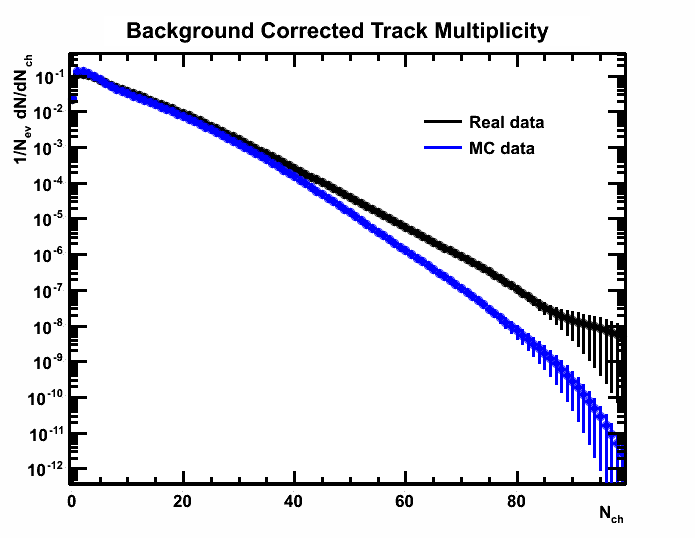
\includegraphics[width=\textwidth]{Chapters/multiplicity/charged_particle_event_multiplicity/images/background_correction_comparison/2_0-4_5.png}
		\caption{$2.0 \le \eta \le 4.5$}
	\end{subfigure}
	\begin{subfigure}{0.32\textwidth}
		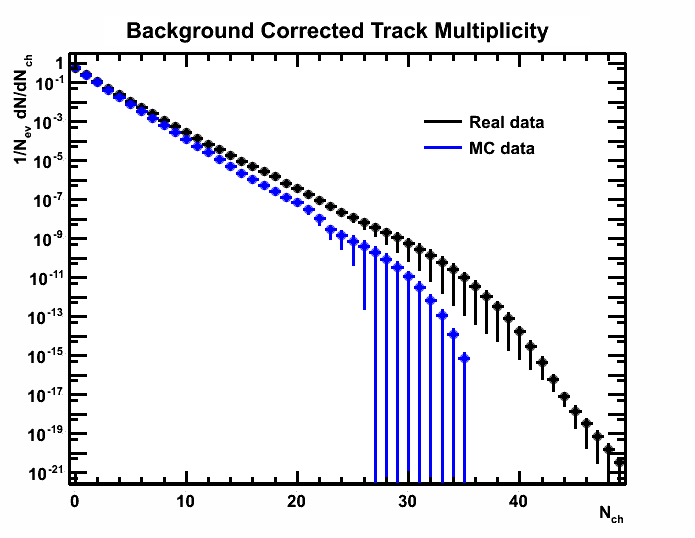
\includegraphics[width=\textwidth]{Chapters/multiplicity/charged_particle_event_multiplicity/images/background_correction_comparison/2_0-2_5.png}
		\caption{$2.0 \le \eta \le 2.5$}
	\end{subfigure}
	\begin{subfigure}{0.32\textwidth}
		\includegraphics[width=\textwidth]{Chapters/multiplicity/charged_particle_event_multiplicity/images/background_correction_comparison/2_5-3_0.png}
		\caption{$2.5 \le \eta \le 3.0$}
	\end{subfigure}
	\begin{subfigure}{0.32\textwidth}
		\includegraphics[width=\textwidth]{Chapters/multiplicity/charged_particle_event_multiplicity/images/background_correction_comparison/3_0-3_5.png}
		\caption{$3.0 \le \eta \le 3.5$}
	\end{subfigure}
	\begin{subfigure}{0.32\textwidth}
		\includegraphics[width=\textwidth]{Chapters/multiplicity/charged_particle_event_multiplicity/images/background_correction_comparison/3_5-4_0.png}
		\caption{$3.5 \le \eta \le 4.0$}
	\end{subfigure}
	\begin{subfigure}{0.32\textwidth}
		\includegraphics[width=\textwidth]{Chapters/multiplicity/charged_particle_event_multiplicity/images/background_correction_comparison/4_0-4_5.png}
		\caption{$4.0 \le \eta \le 4.5$}
	\end{subfigure}
	\caption{Background corrected track multiplicities from measured data and MC}
	\label{fig: background corrected track multiplicity comparison}
\end{figure}

%\begin{figure}[h]
%	\centering
%	\begin{subfigure}{0.32\textwidth}
%		\includegraphics[width=\textwidth]{/afs/cern.ch/user/d/dvoong/cmtuser/DaVinci_v33r6/Phys/ChargedParticleMultiplicity/python/multiplicity/tracks/data_files/TrackMultiplicityPlottingJob/bk/Down/mc/-1/-1/bk/Down/mc/-1/-1/meissner_multiplicity_full/bk/Down/mc/-1/-1/bk/Down/mc/-1/-1/pngs/cross_check/2-0_4-5.png}
%		\caption{$2.0 \le \eta \le 4.5$}
%	\end{subfigure}
%	\begin{subfigure}{0.32\textwidth}
%		\includegraphics[width=\textwidth]{/afs/cern.ch/user/d/dvoong/cmtuser/DaVinci_v33r6/Phys/ChargedParticleMultiplicity/python/multiplicity/tracks/data_files/TrackMultiplicityPlottingJob/bk/Down/mc/-1/-1/bk/Down/mc/-1/-1/meissner_multiplicity/bk/Down/mc/-1/-1/bk/Down/mc/-1/-1/pngs/cross_check/2-0_2-5.png}
%		\caption{$2.0 \le \eta \le 2.5$}
%	\end{subfigure}
%	\begin{subfigure}{0.32\textwidth}
%		\includegraphics[width=\textwidth]{/afs/cern.ch/user/d/dvoong/cmtuser/DaVinci_v33r6/Phys/ChargedParticleMultiplicity/python/multiplicity/tracks/data_files/TrackMultiplicityPlottingJob/bk/Down/mc/-1/-1/bk/Down/mc/-1/-1/meissner_multiplicity/bk/Down/mc/-1/-1/bk/Down/mc/-1/-1/pngs/cross_check/2-5_3-0.png}
%		\caption{$2.5 \le \eta \le 3.0$}
%	\end{subfigure}
%	\begin{subfigure}{0.32\textwidth}
%		\includegraphics[width=\textwidth]{/afs/cern.ch/user/d/dvoong/cmtuser/DaVinci_v33r6/Phys/ChargedParticleMultiplicity/python/multiplicity/tracks/data_files/TrackMultiplicityPlottingJob/bk/Down/mc/-1/-1/bk/Down/mc/-1/-1/meissner_multiplicity/bk/Down/mc/-1/-1/bk/Down/mc/-1/-1/pngs/cross_check/3-0_3-5.png}
%		\caption{$3.0 \le \eta \le 3.5$}
%	\end{subfigure}
%	\begin{subfigure}{0.32\textwidth}
%		\includegraphics[width=\textwidth]{/afs/cern.ch/user/d/dvoong/cmtuser/DaVinci_v33r6/Phys/ChargedParticleMultiplicity/python/multiplicity/tracks/data_files/TrackMultiplicityPlottingJob/bk/Down/mc/-1/-1/bk/Down/mc/-1/-1/meissner_multiplicity/bk/Down/mc/-1/-1/bk/Down/mc/-1/-1/pngs/cross_check/3-5_4-0.png}
%		\caption{$3.5 \le \eta \le 4.0$}
%	\end{subfigure}
%	\begin{subfigure}{0.32\textwidth}
%		\includegraphics[width=\textwidth]{/afs/cern.ch/user/d/dvoong/cmtuser/DaVinci_v33r6/Phys/ChargedParticleMultiplicity/python/multiplicity/tracks/data_files/TrackMultiplicityPlottingJob/bk/Down/mc/-1/-1/bk/Down/mc/-1/-1/meissner_multiplicity/bk/Down/mc/-1/-1/bk/Down/mc/-1/-1/pngs/cross_check/4-0_4-5.png}
%		\caption{$4.0 \le \eta \le 4.5$}
%	\end{subfigure}
%	\caption{Background correction cross-check. Background corrected track multiplicities are compared with tracks matched to generator prompt particles by MC truth matching}
%	\label{fig: background corrected track multiplicity cross-check}
%\end{figure}
%\section{Response Matrix}
\label{section: response matrix}

The response matrix is an n by m matrix $R_{nm}$, each element gives the probability of reconstructing n number of tracks given an event with m number of particles. The relationship between the reconstructed track multiplicity  and true particle distribution ($a$) is described by the equation,

\begin{equation}
	a = R \cdot b
\end{equation} 

where a and b are column matrices describing the track and particle multiplicities respectively such that $a_i$ is the number of events with $i$ reconstructed tracks and $b_j$ is the number of events with $j$ corresponding true particles.

The response matrix is determined using truth information from Monte Carlo simulated events. 

\begin{figure}
	\centering
	\begin{subfigure}{0.32\textwidth}
		\includegraphics[width=\textwidth]{/afs/cern.ch/user/d/dvoong/cmtuser/DaVinci_v33r6/Phys/ChargedParticleMultiplicity/python/response_matrix/data_files/ResponseMatrixPlottingJob/bk/Down/mc/-1/-1/bk/Down/mc/-1/-1/meissner_multiplicity_full/bk/Down/mc/-1/-1/bk/Down/mc/-1/-1/pngs/background_corrected/2-0_4-5.png}
		\caption{$2.0 \le \eta \le 4.5$}
	\end{subfigure}
	\begin{subfigure}{0.32\textwidth}
		\includegraphics[width=\textwidth]{/afs/cern.ch/user/d/dvoong/cmtuser/DaVinci_v33r6/Phys/ChargedParticleMultiplicity/python/response_matrix/data_files/ResponseMatrixPlottingJob/bk/Down/mc/-1/-1/bk/Down/mc/-1/-1/meissner_multiplicity/bk/Down/mc/-1/-1/bk/Down/mc/-1/-1/pngs/background_corrected/2-0_2-5.png}
		\caption{$2.0 \le \eta \le 2.5$}
	\end{subfigure}
	\begin{subfigure}{0.32\textwidth}
		\includegraphics[width=\textwidth]{/afs/cern.ch/user/d/dvoong/cmtuser/DaVinci_v33r6/Phys/ChargedParticleMultiplicity/python/response_matrix/data_files/ResponseMatrixPlottingJob/bk/Down/mc/-1/-1/bk/Down/mc/-1/-1/meissner_multiplicity/bk/Down/mc/-1/-1/bk/Down/mc/-1/-1/pngs/background_corrected/2-5_3-0.png}
		\caption{$2.5 \le \eta \le 3.0$}
	\end{subfigure}
	\begin{subfigure}{0.32\textwidth}
		\includegraphics[width=\textwidth]{/afs/cern.ch/user/d/dvoong/cmtuser/DaVinci_v33r6/Phys/ChargedParticleMultiplicity/python/response_matrix/data_files/ResponseMatrixPlottingJob/bk/Down/mc/-1/-1/bk/Down/mc/-1/-1/meissner_multiplicity/bk/Down/mc/-1/-1/bk/Down/mc/-1/-1/pngs/background_corrected/3-0_3-5.png}
		\caption{$3.0 \le \eta \le 3.5$}
	\end{subfigure}
	\begin{subfigure}{0.32\textwidth}
		\includegraphics[width=\textwidth]{/afs/cern.ch/user/d/dvoong/cmtuser/DaVinci_v33r6/Phys/ChargedParticleMultiplicity/python/response_matrix/data_files/ResponseMatrixPlottingJob/bk/Down/mc/-1/-1/bk/Down/mc/-1/-1/meissner_multiplicity/bk/Down/mc/-1/-1/bk/Down/mc/-1/-1/pngs/background_corrected/3-5_4-0.png}
		\caption{$3.5 \le \eta \le 4.0$}
	\end{subfigure}
	\begin{subfigure}{0.32\textwidth}
		\includegraphics[width=\textwidth]{/afs/cern.ch/user/d/dvoong/cmtuser/DaVinci_v33r6/Phys/ChargedParticleMultiplicity/python/response_matrix/data_files/ResponseMatrixPlottingJob/bk/Down/mc/-1/-1/bk/Down/mc/-1/-1/meissner_multiplicity/bk/Down/mc/-1/-1/bk/Down/mc/-1/-1/pngs/background_corrected/4-0_4-5.png}
		\caption{$4.0 \le \eta \le 4.5$}
	\end{subfigure}
	\caption{Background corrected response matrices}
	\label{fig: background corrected response matrices}
\end{figure}
%\subsubsection{True Multiplicity Parameterisation}
\label{subsection: charged particle event multiplicity, true multiplicity parameterisation}

Starting from equation \ref{equation: multiplicity-response relationship} a heuristic approach to calculating the true particle multiplicity can be employed. By making a educated guess at the shape of the true distribution a corresponding expected multiplicity can be calculated by applying the response matrix. Comparing the observed multiplicity to the expected multiplicity gives a quantifiable measurement of the accuracy of the guess. To achieve this in a more systematic way, a parameterisation of the true distribution ($b'$) can be made for which a corresponding response (or smearing) functions ($a'$) exists. By fitting the response function to the observed multiplicity the associated parameters can be propagated back in terms of the parameterisation of the true multiplicity distribution to give a corrected multiplicity distribution. The response function and corresponding $\chi^2$ minimisation function that were used are,

\begin{equation}
	a'(p_0, p_1, ..., p_n) = R \cdot b'(p_0, p_1, ..., p_n)
\end{equation}

\begin{equation}
	\chi^2(p_0, p_1, ..., p_n) = \sum^{N_\mathrm{max}}_{N_\mathrm{ch}} \sqrt{a(N_\mathrm{ch})^2 - a'(N_\mathrm{ch})^2}
	\label{equation: response function minimisation}
\end{equation}

Where $p_0, p_1, ..., p_n$ corresponds to the parameters used to parameterise the response function and hence true multiplicity, $N_\mathrm{max}$ is the maximum number of reconstructed tracks ($N_\mathrm{ch}$), $a(N_\mathrm{ch})$ is the number of events with $N_\mathrm{ch}$ tracks and $a'(N_\mathrm{ch})$ is the number of events with $N_\mathrm{ch}$ reconstructed tracks predicted by the response function.

%The true multiplicity is parameterised using several functions in order to optimise the robustness of the unfolding procedure.
%The following parameterisation functions were used,

The true multiplicity distribution is parameterised by several parameterisations (listed below). These parameterisations consist of several parameters such that the parameterisations are extremely flexible and robust. This enables the parameterisations to model a range of possible true distributions, minimising the bias associated to modelling an unknown distribution. The initial values of the parameters in each parameterisation are initialised by fitting MC generated data with each parameterisations, the fits are shown in figure \ref{fig: parameterisation fits} and the parameters are shown in table \ref{table: gen multiplicity parameters}.

\begin{itemize}
	\item $P_A(x) = p_0 e^{p_1x}x^2 + e^{p_2x}x^2$
	\item $P_B(x) = e^{p_0 + p_1x} \cdot (x + 1)^3 + e^{p_2 + p_3x} \cdot x^2 + e^{p_4 + p_5x} \cdot x^2$
%	\item $P_C(x) = \mathrm{NBD}(x; p_0, p_1) + p_6 \mathrm{NBD}(x + p_8; p_2, p_3) + p_7 \mathrm{NBD}(x + p_9; p_4, p_5)$
	\item $P_C(x) = e^{p_0 + p_1x} \cdot x^{p_2} + e^{p_3 + p_4x} \cdot x^{p_5} + e^{p_6 + p_7x} \cdot x^{p_8}$
%	\item $P_D(x) = e^{p_0 + p_1 \cdot x^{p_2}} \cdot x^2 + e^{p_3 + p_4x + p_5(p_7x)^{p_6}} + \frac{p_8}{x+1} \cdot e^\frac{p9}{x+1}$
	\item $P_E(x) = e^{p_0 + p_1x} \cdot x^{p_2} + e^{p_3 + p_4x} \cdot x^2$
\end{itemize}

%\begin{equation}
%	f(x) = p_0 e^{p_1x}x^2 + e^{p_2x}x^2
%\end{equation}
%
%\begin{equation}
%	f(x) = e^{p_0 + p_1x} \cdot (x + 1)^3 + e^{p_2 + p_3x} \cdot x^2 + e^{p_4 + p_5x} \cdot x^2
%\end{equation}
%
%\begin{equation}
%	f(x) = \frac{n!}{x!(n-x)!} \cdot p^x \cdot (1-p)^{n-x} + p_6 \cdot \left( \frac{n'!}{x!(n'-x)!} \cdot p'^x \cdot(1-p')^{n'-x} \right) + p_7 \cdot \left( \frac{n''!}{(x+1)!(n''-x)!} \cdot p''^{x + 1} \cdot (1-p'')^{(n'' - (x+1))} \right)
%\end{equation}
%
%\begin{equation}
%	f(x) = e^{p_0 + p_1x} \cdot x^{p_2} + e^{p_3 + p_4x} \cdot x^{p_5} + e^{p_6 + p_7x} \cdot x^{p_8}
%\end{equation}
%
%\begin{equation}
%	f(x) = e^{p_0 + p_1 \cdot x^{p_2}} \cdot x^2 + e^{p_3 + p_4x + p_5(p_7x)^{p_6}} + \frac{p_8}{x+1} \cdot e^\frac{p9}{x+1}
%\end{equation}
%
%\begin{equation}
%	f(x) = e^{p_0 + p_1x} \cdot x^{p_2} + e^{p_3 + p_4x} \cdot x^2
%\end{equation}

%Due to the non-perturbative nature of the multiplicity distribution there is ambiguity in the shape of the multiplicity distribution. These parameterisation functions are adopted in order to give a high degree of flexibility and robustness in describing the multiplicity distribution.

\begin{figure}[H]
	\centering
	\begin{subfigure}{0.49\textwidth}
		\includegraphics[width=\textwidth]{/afs/cern.ch/user/d/dvoong/cmtuser/DaVinci_v33r6/Phys/ChargedParticleMultiplicity/python/multiplicity/genps/parameterisation/data_files/GenpMultiplicityParameterisationPlottingJob/bk/Down/mc/-1/-1/bk/Down/mc/-1/155/parameterisation_a/2_0-4_5/parameterisation_a.png}
		\caption{Parameterisation A}
		\label{}
	\end{subfigure}
	\begin{subfigure}{0.49\textwidth}
		\includegraphics[width=\textwidth]{/afs/cern.ch/user/d/dvoong/cmtuser/DaVinci_v33r6/Phys/ChargedParticleMultiplicity/python/multiplicity/genps/parameterisation/data_files/GenpMultiplicityParameterisationPlottingJob/bk/Down/mc/-1/-1/bk/Down/mc/-1/155/parameterisation_b/2_0-4_5/parameterisation_b.png}
		\caption{Parameterisation B}
		\label{}
	\end{subfigure}
%	\begin{subfigure}{0.49\textwidth}
%		\includegraphics[width=\textwidth]{/afs/cern.ch/user/d/dvoong/cmtuser/DaVinci_v33r6/Phys/ChargedParticleMultiplicity/python/multiplicity/genps/parameterisation/data_files/GenpMultiplicityParameterisationPlottingJob/bk/Down/mc/-1/-1/bk/Down/mc/-1/155/parameterisation_c/2_0-4_5/parameterisation_c.png}
%		\caption{Parameterisation C}
%		\label{}
%	\end{subfigure}
	\begin{subfigure}{0.49\textwidth}
		\includegraphics[width=\textwidth]{/afs/cern.ch/user/d/dvoong/cmtuser/DaVinci_v33r6/Phys/ChargedParticleMultiplicity/python/multiplicity/genps/parameterisation/data_files/GenpMultiplicityParameterisationPlottingJob/bk/Down/mc/-1/-1/bk/Down/mc/-1/155/parameterisation_d/2_0-4_5/parameterisation_d.png}
		\caption{Parameterisation D}
		\label{}
	\end{subfigure}
%	\begin{subfigure}{0.49\textwidth}
%		\includegraphics[width=\textwidth]{/afs/cern.ch/user/d/dvoong/cmtuser/DaVinci_v33r6/Phys/ChargedParticleMultiplicity/python/multiplicity/genps/parameterisation/data_files/GenpMultiplicityParameterisationPlottingJob/bk/Down/mc/-1/-1/bk/Down/mc/-1/155/parameterisation_e/2_0-4_5/parameterisation_e.png}
%		\caption{Parameterisation E}
%		\label{}
%	\end{subfigure}
	\begin{subfigure}{0.49\textwidth}
		\includegraphics[width=\textwidth]{/afs/cern.ch/user/d/dvoong/cmtuser/DaVinci_v33r6/Phys/ChargedParticleMultiplicity/python/multiplicity/genps/parameterisation/data_files/GenpMultiplicityParameterisationPlottingJob/bk/Down/mc/-1/-1/bk/Down/mc/-1/155/parameterisation_f/2_0-4_5/parameterisation_f.png}
		\caption{Parameterisation F}
		\label{}
	\end{subfigure}
	\caption{Parameterisation fits to MC data for $2.0 \le \eta \le 4.5$. The solid blue line corresponds to the total fit and the dotted lines correspond to the components of the total fit}
	\label{fig: parameterisation fits}
\end{figure}

\newpage
\begin{table}[h]
	\caption{True multiplicity parameterisations fit to generated prompt particle distributions}
	\label{table: gen multiplicity parameters}
	\begin{subtable}{0.49\textwidth}
		\caption{Parameterisation A}
		\centering
		\begin{tabular}{|c|c|}
			\centering
			p0 & $14.414 \pm 0.988$ \\
			p1 & $-0.19995 \pm 0.181$ \\
			p2 & $17.887 \pm 0.989$ \\
			p3 & $-0.60499 \pm 0.832$ \\
			p4 & $0.01735 \pm 0.332$ \\
			p5 & $1.5373 \pm 0.998$ \\
			p6 & $1.3577 \pm 1.0$ \\
		\end{tabular}
	\end{subtable}
	\begin{subtable}{0.49\textwidth}
		\caption{Parameterisation B}
		\centering
		\begin{tabular}{|c|c|}
			\centering
			p0 & $-4.4678 \pm 33.9$ \\
			p1 & $-0.66946 \pm 2.78$ \\
			p2 & $-2.7404 \pm 53.7$ \\
			p3 & $-1.0328 \pm 11.9$ \\
			p4 & $-6.0631 \pm 33.0$ \\
			p5 & $-0.19869 \pm 0.323$ \\
		\end{tabular}
	\end{subtable}
%	\begin{subtable}{0.49\textwidth}
%		\caption{Parameterisation C}
%		\centering
%		\begin{tabular}{|c|c|}
%			\centering
%			p0 & $1.1237 \pm 3.91$ \\
%			p1 & $0.090301 \pm 0.76$ \\
%			p2 & $23.184 \pm 6.7e+02$ \\
%			p3 & $0.84887 \pm 0.618$ \\
%			p4 & $4.2472 \pm 43.1$ \\
%			p5 & $0.12728 \pm 0.628$ \\
%			p6 & $0.20308 \pm 0.662$ \\
%			p7 & $-0.10058 \pm 1.45$ \\
%		\end{tabular}
%	\end{subtable}
	\begin{subtable}{0.49\textwidth}
		\caption{Parameterisation D}
		\centering
		\begin{tabular}{|c|c|}
			\centering
			p0 & $-17.893 \pm 1.0$ \\
			p1 & $-0.33501 \pm 0.198$ \\
			p2 & $4.1461 \pm 1.04$ \\
			p3 & $-9.5155 \pm 0.993$ \\
			p4 & $-0.22568 \pm 0.178$ \\
			p5 & $3.1305 \pm 0.962$ \\
			p6 & $-2.5895 \pm 0.994$ \\
			p7 & $-0.37285 \pm 0.531$ \\
			p8 & $1.1071 \pm 0.97$ \\
		\end{tabular}
	\end{subtable}
%	\begin{subtable}{0.49\textwidth}
%		\caption{Parameterisation E}
%		\centering
%		\begin{tabular}{|c|c|}
%			\centering
%			p0 & $-6.9649 \pm 11.9$ \\
%			p1 & $-0.1352 \pm 0.302$ \\
%			p2 & $1.074 \pm 0.559$ \\
%			p3 & $16.049 \pm 11.8$ \\
%			p4 & $-0.39655 \pm 0.912$ \\
%			p5 & $-9.7608 \pm 6.69$ \\
%			p6 & $-0.066749 \pm 0.0762$ \\
%			p7 & $7.3009e-05 \pm 0.000732$ \\
%			p8 & $-101.39 \pm 6.09e+04$ \\
%			p9 & $-837.68 \pm 4.06e+04$ \\
%		\end{tabular}
%	\end{subtable}
	\begin{subtable}{0.49\textwidth}
		\caption{Parameterisation F}
		\centering
		\begin{tabular}{|c|c|}
			\centering
			p0 & $-6.3713 \pm 33.5$ \\
			p1 & $-0.20009 \pm 0.272$ \\
			p2 & $-2.6787 \pm 33.5$ \\
			p3 & $-0.6491 \pm 1.08$ \\
		\end{tabular}
	\end{subtable}
\end{table}
\newpage
\subsection{Efficiency Correction}
\label{subsection: charged particle multiplicity, efficiency correction}

\section{Response Matrix}
\label{section: response matrix}

The response matrix is an n by m matrix $R_{nm}$, each element gives the probability of reconstructing n number of tracks given an event with m number of particles. The relationship between the reconstructed track multiplicity  and true particle distribution ($a$) is described by the equation,

\begin{equation}
	a = R \cdot b
\end{equation} 

where a and b are column matrices describing the track and particle multiplicities respectively such that $a_i$ is the number of events with $i$ reconstructed tracks and $b_j$ is the number of events with $j$ corresponding true particles.

The response matrix is determined using truth information from Monte Carlo simulated events. 

\begin{figure}
	\centering
	\begin{subfigure}{0.32\textwidth}
		\includegraphics[width=\textwidth]{/afs/cern.ch/user/d/dvoong/cmtuser/DaVinci_v33r6/Phys/ChargedParticleMultiplicity/python/response_matrix/data_files/ResponseMatrixPlottingJob/bk/Down/mc/-1/-1/bk/Down/mc/-1/-1/meissner_multiplicity_full/bk/Down/mc/-1/-1/bk/Down/mc/-1/-1/pngs/background_corrected/2-0_4-5.png}
		\caption{$2.0 \le \eta \le 4.5$}
	\end{subfigure}
	\begin{subfigure}{0.32\textwidth}
		\includegraphics[width=\textwidth]{/afs/cern.ch/user/d/dvoong/cmtuser/DaVinci_v33r6/Phys/ChargedParticleMultiplicity/python/response_matrix/data_files/ResponseMatrixPlottingJob/bk/Down/mc/-1/-1/bk/Down/mc/-1/-1/meissner_multiplicity/bk/Down/mc/-1/-1/bk/Down/mc/-1/-1/pngs/background_corrected/2-0_2-5.png}
		\caption{$2.0 \le \eta \le 2.5$}
	\end{subfigure}
	\begin{subfigure}{0.32\textwidth}
		\includegraphics[width=\textwidth]{/afs/cern.ch/user/d/dvoong/cmtuser/DaVinci_v33r6/Phys/ChargedParticleMultiplicity/python/response_matrix/data_files/ResponseMatrixPlottingJob/bk/Down/mc/-1/-1/bk/Down/mc/-1/-1/meissner_multiplicity/bk/Down/mc/-1/-1/bk/Down/mc/-1/-1/pngs/background_corrected/2-5_3-0.png}
		\caption{$2.5 \le \eta \le 3.0$}
	\end{subfigure}
	\begin{subfigure}{0.32\textwidth}
		\includegraphics[width=\textwidth]{/afs/cern.ch/user/d/dvoong/cmtuser/DaVinci_v33r6/Phys/ChargedParticleMultiplicity/python/response_matrix/data_files/ResponseMatrixPlottingJob/bk/Down/mc/-1/-1/bk/Down/mc/-1/-1/meissner_multiplicity/bk/Down/mc/-1/-1/bk/Down/mc/-1/-1/pngs/background_corrected/3-0_3-5.png}
		\caption{$3.0 \le \eta \le 3.5$}
	\end{subfigure}
	\begin{subfigure}{0.32\textwidth}
		\includegraphics[width=\textwidth]{/afs/cern.ch/user/d/dvoong/cmtuser/DaVinci_v33r6/Phys/ChargedParticleMultiplicity/python/response_matrix/data_files/ResponseMatrixPlottingJob/bk/Down/mc/-1/-1/bk/Down/mc/-1/-1/meissner_multiplicity/bk/Down/mc/-1/-1/bk/Down/mc/-1/-1/pngs/background_corrected/3-5_4-0.png}
		\caption{$3.5 \le \eta \le 4.0$}
	\end{subfigure}
	\begin{subfigure}{0.32\textwidth}
		\includegraphics[width=\textwidth]{/afs/cern.ch/user/d/dvoong/cmtuser/DaVinci_v33r6/Phys/ChargedParticleMultiplicity/python/response_matrix/data_files/ResponseMatrixPlottingJob/bk/Down/mc/-1/-1/bk/Down/mc/-1/-1/meissner_multiplicity/bk/Down/mc/-1/-1/bk/Down/mc/-1/-1/pngs/background_corrected/4-0_4-5.png}
		\caption{$4.0 \le \eta \le 4.5$}
	\end{subfigure}
	\caption{Background corrected response matrices}
	\label{fig: background corrected response matrices}
\end{figure}
\subsubsection{True Multiplicity Parameterisation}
\label{subsection: charged particle event multiplicity, true multiplicity parameterisation}

Starting from equation \ref{equation: multiplicity-response relationship} a heuristic approach to calculating the true particle multiplicity can be employed. By making a educated guess at the shape of the true distribution a corresponding expected multiplicity can be calculated by applying the response matrix. Comparing the observed multiplicity to the expected multiplicity gives a quantifiable measurement of the accuracy of the guess. To achieve this in a more systematic way, a parameterisation of the true distribution ($b'$) can be made for which a corresponding response (or smearing) functions ($a'$) exists. By fitting the response function to the observed multiplicity the associated parameters can be propagated back in terms of the parameterisation of the true multiplicity distribution to give a corrected multiplicity distribution. The response function and corresponding $\chi^2$ minimisation function that were used are,

\begin{equation}
	a'(p_0, p_1, ..., p_n) = R \cdot b'(p_0, p_1, ..., p_n)
\end{equation}

\begin{equation}
	\chi^2(p_0, p_1, ..., p_n) = \sum^{N_\mathrm{max}}_{N_\mathrm{ch}} \sqrt{a(N_\mathrm{ch})^2 - a'(N_\mathrm{ch})^2}
	\label{equation: response function minimisation}
\end{equation}

Where $p_0, p_1, ..., p_n$ corresponds to the parameters used to parameterise the response function and hence true multiplicity, $N_\mathrm{max}$ is the maximum number of reconstructed tracks ($N_\mathrm{ch}$), $a(N_\mathrm{ch})$ is the number of events with $N_\mathrm{ch}$ tracks and $a'(N_\mathrm{ch})$ is the number of events with $N_\mathrm{ch}$ reconstructed tracks predicted by the response function.

%The true multiplicity is parameterised using several functions in order to optimise the robustness of the unfolding procedure.
%The following parameterisation functions were used,

The true multiplicity distribution is parameterised by several parameterisations (listed below). These parameterisations consist of several parameters such that the parameterisations are extremely flexible and robust. This enables the parameterisations to model a range of possible true distributions, minimising the bias associated to modelling an unknown distribution. The initial values of the parameters in each parameterisation are initialised by fitting MC generated data with each parameterisations, the fits are shown in figure \ref{fig: parameterisation fits} and the parameters are shown in table \ref{table: gen multiplicity parameters}.

\begin{itemize}
	\item $P_A(x) = p_0 e^{p_1x}x^2 + e^{p_2x}x^2$
	\item $P_B(x) = e^{p_0 + p_1x} \cdot (x + 1)^3 + e^{p_2 + p_3x} \cdot x^2 + e^{p_4 + p_5x} \cdot x^2$
%	\item $P_C(x) = \mathrm{NBD}(x; p_0, p_1) + p_6 \mathrm{NBD}(x + p_8; p_2, p_3) + p_7 \mathrm{NBD}(x + p_9; p_4, p_5)$
	\item $P_C(x) = e^{p_0 + p_1x} \cdot x^{p_2} + e^{p_3 + p_4x} \cdot x^{p_5} + e^{p_6 + p_7x} \cdot x^{p_8}$
%	\item $P_D(x) = e^{p_0 + p_1 \cdot x^{p_2}} \cdot x^2 + e^{p_3 + p_4x + p_5(p_7x)^{p_6}} + \frac{p_8}{x+1} \cdot e^\frac{p9}{x+1}$
	\item $P_E(x) = e^{p_0 + p_1x} \cdot x^{p_2} + e^{p_3 + p_4x} \cdot x^2$
\end{itemize}

%\begin{equation}
%	f(x) = p_0 e^{p_1x}x^2 + e^{p_2x}x^2
%\end{equation}
%
%\begin{equation}
%	f(x) = e^{p_0 + p_1x} \cdot (x + 1)^3 + e^{p_2 + p_3x} \cdot x^2 + e^{p_4 + p_5x} \cdot x^2
%\end{equation}
%
%\begin{equation}
%	f(x) = \frac{n!}{x!(n-x)!} \cdot p^x \cdot (1-p)^{n-x} + p_6 \cdot \left( \frac{n'!}{x!(n'-x)!} \cdot p'^x \cdot(1-p')^{n'-x} \right) + p_7 \cdot \left( \frac{n''!}{(x+1)!(n''-x)!} \cdot p''^{x + 1} \cdot (1-p'')^{(n'' - (x+1))} \right)
%\end{equation}
%
%\begin{equation}
%	f(x) = e^{p_0 + p_1x} \cdot x^{p_2} + e^{p_3 + p_4x} \cdot x^{p_5} + e^{p_6 + p_7x} \cdot x^{p_8}
%\end{equation}
%
%\begin{equation}
%	f(x) = e^{p_0 + p_1 \cdot x^{p_2}} \cdot x^2 + e^{p_3 + p_4x + p_5(p_7x)^{p_6}} + \frac{p_8}{x+1} \cdot e^\frac{p9}{x+1}
%\end{equation}
%
%\begin{equation}
%	f(x) = e^{p_0 + p_1x} \cdot x^{p_2} + e^{p_3 + p_4x} \cdot x^2
%\end{equation}

%Due to the non-perturbative nature of the multiplicity distribution there is ambiguity in the shape of the multiplicity distribution. These parameterisation functions are adopted in order to give a high degree of flexibility and robustness in describing the multiplicity distribution.

\begin{figure}[H]
	\centering
	\begin{subfigure}{0.49\textwidth}
		\includegraphics[width=\textwidth]{/afs/cern.ch/user/d/dvoong/cmtuser/DaVinci_v33r6/Phys/ChargedParticleMultiplicity/python/multiplicity/genps/parameterisation/data_files/GenpMultiplicityParameterisationPlottingJob/bk/Down/mc/-1/-1/bk/Down/mc/-1/155/parameterisation_a/2_0-4_5/parameterisation_a.png}
		\caption{Parameterisation A}
		\label{}
	\end{subfigure}
	\begin{subfigure}{0.49\textwidth}
		\includegraphics[width=\textwidth]{/afs/cern.ch/user/d/dvoong/cmtuser/DaVinci_v33r6/Phys/ChargedParticleMultiplicity/python/multiplicity/genps/parameterisation/data_files/GenpMultiplicityParameterisationPlottingJob/bk/Down/mc/-1/-1/bk/Down/mc/-1/155/parameterisation_b/2_0-4_5/parameterisation_b.png}
		\caption{Parameterisation B}
		\label{}
	\end{subfigure}
%	\begin{subfigure}{0.49\textwidth}
%		\includegraphics[width=\textwidth]{/afs/cern.ch/user/d/dvoong/cmtuser/DaVinci_v33r6/Phys/ChargedParticleMultiplicity/python/multiplicity/genps/parameterisation/data_files/GenpMultiplicityParameterisationPlottingJob/bk/Down/mc/-1/-1/bk/Down/mc/-1/155/parameterisation_c/2_0-4_5/parameterisation_c.png}
%		\caption{Parameterisation C}
%		\label{}
%	\end{subfigure}
	\begin{subfigure}{0.49\textwidth}
		\includegraphics[width=\textwidth]{/afs/cern.ch/user/d/dvoong/cmtuser/DaVinci_v33r6/Phys/ChargedParticleMultiplicity/python/multiplicity/genps/parameterisation/data_files/GenpMultiplicityParameterisationPlottingJob/bk/Down/mc/-1/-1/bk/Down/mc/-1/155/parameterisation_d/2_0-4_5/parameterisation_d.png}
		\caption{Parameterisation D}
		\label{}
	\end{subfigure}
%	\begin{subfigure}{0.49\textwidth}
%		\includegraphics[width=\textwidth]{/afs/cern.ch/user/d/dvoong/cmtuser/DaVinci_v33r6/Phys/ChargedParticleMultiplicity/python/multiplicity/genps/parameterisation/data_files/GenpMultiplicityParameterisationPlottingJob/bk/Down/mc/-1/-1/bk/Down/mc/-1/155/parameterisation_e/2_0-4_5/parameterisation_e.png}
%		\caption{Parameterisation E}
%		\label{}
%	\end{subfigure}
	\begin{subfigure}{0.49\textwidth}
		\includegraphics[width=\textwidth]{/afs/cern.ch/user/d/dvoong/cmtuser/DaVinci_v33r6/Phys/ChargedParticleMultiplicity/python/multiplicity/genps/parameterisation/data_files/GenpMultiplicityParameterisationPlottingJob/bk/Down/mc/-1/-1/bk/Down/mc/-1/155/parameterisation_f/2_0-4_5/parameterisation_f.png}
		\caption{Parameterisation F}
		\label{}
	\end{subfigure}
	\caption{Parameterisation fits to MC data for $2.0 \le \eta \le 4.5$. The solid blue line corresponds to the total fit and the dotted lines correspond to the components of the total fit}
	\label{fig: parameterisation fits}
\end{figure}

\newpage
\begin{table}[h]
	\caption{True multiplicity parameterisations fit to generated prompt particle distributions}
	\label{table: gen multiplicity parameters}
	\begin{subtable}{0.49\textwidth}
		\caption{Parameterisation A}
		\centering
		\begin{tabular}{|c|c|}
			\centering
			p0 & $14.414 \pm 0.988$ \\
			p1 & $-0.19995 \pm 0.181$ \\
			p2 & $17.887 \pm 0.989$ \\
			p3 & $-0.60499 \pm 0.832$ \\
			p4 & $0.01735 \pm 0.332$ \\
			p5 & $1.5373 \pm 0.998$ \\
			p6 & $1.3577 \pm 1.0$ \\
		\end{tabular}
	\end{subtable}
	\begin{subtable}{0.49\textwidth}
		\caption{Parameterisation B}
		\centering
		\begin{tabular}{|c|c|}
			\centering
			p0 & $-4.4678 \pm 33.9$ \\
			p1 & $-0.66946 \pm 2.78$ \\
			p2 & $-2.7404 \pm 53.7$ \\
			p3 & $-1.0328 \pm 11.9$ \\
			p4 & $-6.0631 \pm 33.0$ \\
			p5 & $-0.19869 \pm 0.323$ \\
		\end{tabular}
	\end{subtable}
%	\begin{subtable}{0.49\textwidth}
%		\caption{Parameterisation C}
%		\centering
%		\begin{tabular}{|c|c|}
%			\centering
%			p0 & $1.1237 \pm 3.91$ \\
%			p1 & $0.090301 \pm 0.76$ \\
%			p2 & $23.184 \pm 6.7e+02$ \\
%			p3 & $0.84887 \pm 0.618$ \\
%			p4 & $4.2472 \pm 43.1$ \\
%			p5 & $0.12728 \pm 0.628$ \\
%			p6 & $0.20308 \pm 0.662$ \\
%			p7 & $-0.10058 \pm 1.45$ \\
%		\end{tabular}
%	\end{subtable}
	\begin{subtable}{0.49\textwidth}
		\caption{Parameterisation D}
		\centering
		\begin{tabular}{|c|c|}
			\centering
			p0 & $-17.893 \pm 1.0$ \\
			p1 & $-0.33501 \pm 0.198$ \\
			p2 & $4.1461 \pm 1.04$ \\
			p3 & $-9.5155 \pm 0.993$ \\
			p4 & $-0.22568 \pm 0.178$ \\
			p5 & $3.1305 \pm 0.962$ \\
			p6 & $-2.5895 \pm 0.994$ \\
			p7 & $-0.37285 \pm 0.531$ \\
			p8 & $1.1071 \pm 0.97$ \\
		\end{tabular}
	\end{subtable}
%	\begin{subtable}{0.49\textwidth}
%		\caption{Parameterisation E}
%		\centering
%		\begin{tabular}{|c|c|}
%			\centering
%			p0 & $-6.9649 \pm 11.9$ \\
%			p1 & $-0.1352 \pm 0.302$ \\
%			p2 & $1.074 \pm 0.559$ \\
%			p3 & $16.049 \pm 11.8$ \\
%			p4 & $-0.39655 \pm 0.912$ \\
%			p5 & $-9.7608 \pm 6.69$ \\
%			p6 & $-0.066749 \pm 0.0762$ \\
%			p7 & $7.3009e-05 \pm 0.000732$ \\
%			p8 & $-101.39 \pm 6.09e+04$ \\
%			p9 & $-837.68 \pm 4.06e+04$ \\
%		\end{tabular}
%	\end{subtable}
	\begin{subtable}{0.49\textwidth}
		\caption{Parameterisation F}
		\centering
		\begin{tabular}{|c|c|}
			\centering
			p0 & $-6.3713 \pm 33.5$ \\
			p1 & $-0.20009 \pm 0.272$ \\
			p2 & $-2.6787 \pm 33.5$ \\
			p3 & $-0.6491 \pm 1.08$ \\
		\end{tabular}
	\end{subtable}
\end{table}
\newpage

%The response functions for the background corrected multiplicities in figure \ref{fig: background corrected track multiplicities} and parameterisations in figure \ref{fig: parameterisation fits} are shown in figure \ref{fig: response function, measured data} and \ref{fig: response function, mc data} for measured and MC data. The corresponding unfolded multiplicities are shown figure \ref{fig: unfolded multiplicity, measured data} and \ref{fig: unfolded multiplicity, mc data} respectively.

The response functions for the background corrected multiplicities in figure \ref{fig: background corrected track multiplicities} and parameterisations in figure \ref{fig: parameterisation fits} are shown in figure \ref{fig: response function, measured data} for measured data. The corresponding unfolded multiplicities are shown figure \ref{fig: unfolded multiplicity, measured data}.

\begin{figure}[H]
	\centering
	\begin{subfigure}{0.49\textwidth}
		\includegraphics[width=\textwidth]{/afs/cern.ch/user/d/dvoong/cmtuser/DaVinci_v33r6/Phys/ChargedParticleMultiplicity/python/multiplicity/tracks/unfolding/data_files/UnfoldingPlottingWithStatsJob/bk/Down/mc/-1/-1/bk/Down/mc/-1/-1/meissner_multiplicity_full/bk/Down/real/-1/-1/bk/Down/real/-1/-1/bk/Down/mc/-1/-1/bk/Down/mc/-1/155/parameterisation_a/2_0-4_5/bk/Down/mc/-1/-1/bk/Down/mc/-1/-1/meissner_multiplicity_full/bk/Down/mc/-1/-1/bk/Down/mc/-1/-1/background_corrected/truncation/response_function.png}
		\caption{Parameterisation A}
	\end{subfigure}
	\begin{subfigure}{0.49\textwidth}
		\includegraphics[width=\textwidth]{/afs/cern.ch/user/d/dvoong/cmtuser/DaVinci_v33r6/Phys/ChargedParticleMultiplicity/python/multiplicity/tracks/unfolding/data_files/UnfoldingPlottingWithStatsJob/bk/Down/mc/-1/-1/bk/Down/mc/-1/-1/meissner_multiplicity_full/bk/Down/real/-1/-1/bk/Down/real/-1/-1/bk/Down/mc/-1/-1/bk/Down/mc/-1/155/parameterisation_b/2_0-4_5/bk/Down/mc/-1/-1/bk/Down/mc/-1/-1/meissner_multiplicity_full/bk/Down/mc/-1/-1/bk/Down/mc/-1/-1/background_corrected/truncation/response_function.png}
		\caption{Parameterisation B}
	\end{subfigure}
%	\begin{subfigure}{0.49\textwidth}
%		\includegraphics[width=\textwidth]{/afs/cern.ch/user/d/dvoong/cmtuser/DaVinci_v33r6/Phys/ChargedParticleMultiplicity/python/multiplicity/tracks/unfolding/data_files/UnfoldingPlottingWithStatsJob/bk/Down/mc/-1/-1/bk/Down/mc/-1/-1/meissner_multiplicity_full/bk/Down/real/-1/-1/bk/Down/real/-1/-1/bk/Down/mc/-1/-1/bk/Down/mc/-1/155/parameterisation_c/2_0-4_5/bk/Down/mc/-1/-1/bk/Down/mc/-1/-1/meissner_multiplicity_full/bk/Down/mc/-1/-1/bk/Down/mc/-1/-1/background_corrected/truncation/response_function.png}
%		\caption{Parameterisation C}
%	\end{subfigure}
	\begin{subfigure}{0.49\textwidth}
		\includegraphics[width=\textwidth]{/afs/cern.ch/user/d/dvoong/cmtuser/DaVinci_v33r6/Phys/ChargedParticleMultiplicity/python/multiplicity/tracks/unfolding/data_files/UnfoldingPlottingWithStatsJob/bk/Down/mc/-1/-1/bk/Down/mc/-1/-1/meissner_multiplicity_full/bk/Down/real/-1/-1/bk/Down/real/-1/-1/bk/Down/mc/-1/-1/bk/Down/mc/-1/155/parameterisation_d/2_0-4_5/bk/Down/mc/-1/-1/bk/Down/mc/-1/-1/meissner_multiplicity_full/bk/Down/mc/-1/-1/bk/Down/mc/-1/-1/background_corrected/truncation/response_function.png}
		\caption{Parameterisation D}
	\end{subfigure}
%	\begin{subfigure}{0.49\textwidth}
%		\includegraphics[width=\textwidth]{/afs/cern.ch/user/d/dvoong/cmtuser/DaVinci_v33r6/Phys/ChargedParticleMultiplicity/python/multiplicity/tracks/unfolding/data_files/UnfoldingPlottingWithStatsJob/bk/Down/mc/-1/-1/bk/Down/mc/-1/-1/meissner_multiplicity_full/bk/Down/real/-1/-1/bk/Down/real/-1/-1/bk/Down/mc/-1/-1/bk/Down/mc/-1/155/parameterisation_e/2_0-4_5/bk/Down/mc/-1/-1/bk/Down/mc/-1/-1/meissner_multiplicity_full/bk/Down/mc/-1/-1/bk/Down/mc/-1/-1/background_corrected/truncation/response_function.png}
%		\caption{Parameterisation E}
%	\end{subfigure}
	\begin{subfigure}{0.49\textwidth}
		\includegraphics[width=\textwidth]{/afs/cern.ch/user/d/dvoong/cmtuser/DaVinci_v33r6/Phys/ChargedParticleMultiplicity/python/multiplicity/tracks/unfolding/data_files/UnfoldingPlottingWithStatsJob/bk/Down/mc/-1/-1/bk/Down/mc/-1/-1/meissner_multiplicity_full/bk/Down/real/-1/-1/bk/Down/real/-1/-1/bk/Down/mc/-1/-1/bk/Down/mc/-1/155/parameterisation_f/2_0-4_5/bk/Down/mc/-1/-1/bk/Down/mc/-1/-1/meissner_multiplicity_full/bk/Down/mc/-1/-1/bk/Down/mc/-1/-1/background_corrected/truncation/response_function.png}
		\caption{Parameterisation F}
	\end{subfigure}
	\caption{Response Function for $2.0 \le \eta \le 4.5$, Measured Data}
	\label{fig: response function, measured data}
\end{figure}

%\newpage
\begin{table}
	\centering
	\caption{Response function parameters}
	\label{table: response function parameters}
	\begin{subtable}{0.49\textwidth}
		\centering
		\caption{Parameterisation A}
		\input{/afs/cern.ch/user/d/dvoong/cmtuser/DaVinci_v33r6/Phys/ChargedParticleMultiplicity/python/multiplicity/tracks/unfolding/data_files/UnfoldingPlottingWithStatsJob/bk/Down/mc/-1/-1/bk/Down/mc/-1/-1/meissner_multiplicity_full/bk/Down/mc/-1/-1/bk/Down/mc/-1/155/bk/Down/mc/-1/-1/bk/Down/mc/-1/155/parameterisation_a/2_0-4_5/bk/Down/mc/-1/-1/bk/Down/mc/-1/-1/meissner_multiplicity_full/bk/Down/mc/-1/-1/bk/Down/mc/-1/-1/background_corrected/parameterised/parameters}
	\end{subtable}
	\begin{subtable}{0.49\textwidth}
		\centering
		\caption{Parameterisation B}
		\input{/afs/cern.ch/user/d/dvoong/cmtuser/DaVinci_v33r6/Phys/ChargedParticleMultiplicity/python/multiplicity/tracks/unfolding/data_files/UnfoldingPlottingWithStatsJob/bk/Down/mc/-1/-1/bk/Down/mc/-1/-1/meissner_multiplicity_full/bk/Down/mc/-1/-1/bk/Down/mc/-1/155/bk/Down/mc/-1/-1/bk/Down/mc/-1/155/parameterisation_b/2_0-4_5/bk/Down/mc/-1/-1/bk/Down/mc/-1/-1/meissner_multiplicity_full/bk/Down/mc/-1/-1/bk/Down/mc/-1/-1/background_corrected/parameterised/parameters}
	\end{subtable}
	\begin{subtable}{0.49\textwidth}
		\caption{Parameterisation D}
		\centering
		\input{/afs/cern.ch/user/d/dvoong/cmtuser/DaVinci_v33r6/Phys/ChargedParticleMultiplicity/python/multiplicity/tracks/unfolding/data_files/UnfoldingPlottingWithStatsJob/bk/Down/mc/-1/-1/bk/Down/mc/-1/-1/meissner_multiplicity_full/bk/Down/mc/-1/-1/bk/Down/mc/-1/155/bk/Down/mc/-1/-1/bk/Down/mc/-1/155/parameterisation_d/2_0-4_5/bk/Down/mc/-1/-1/bk/Down/mc/-1/-1/meissner_multiplicity_full/bk/Down/mc/-1/-1/bk/Down/mc/-1/-1/background_corrected/parameterised/parameters}
	\end{subtable}
%	\begin{subtable}{0.49\textwidth}
%		\centering
%		\caption{Parameterisation E}
%		\input{/afs/cern.ch/user/d/dvoong/cmtuser/DaVinci_v33r6/Phys/ChargedParticleMultiplicity/python/multiplicity/tracks/unfolding/data_files/UnfoldingPlottingWithStatsJob/bk/Down/mc/-1/-1/bk/Down/mc/-1/-1/meissner_multiplicity_full/bk/Down/mc/-1/-1/bk/Down/mc/-1/155/bk/Down/mc/-1/-1/bk/Down/mc/-1/155/parameterisation_e/2_0-4_5/bk/Down/mc/-1/-1/bk/Down/mc/-1/-1/meissner_multiplicity_full/bk/Down/mc/-1/-1/bk/Down/mc/-1/-1/background_corrected/parameterised/parameters}
%	\end{subtable}
	\begin{subtable}{0.49\textwidth}
		\centering
		\caption{Parameterisation F}
		\input{/afs/cern.ch/user/d/dvoong/cmtuser/DaVinci_v33r6/Phys/ChargedParticleMultiplicity/python/multiplicity/tracks/unfolding/data_files/UnfoldingPlottingWithStatsJob/bk/Down/mc/-1/-1/bk/Down/mc/-1/-1/meissner_multiplicity_full/bk/Down/mc/-1/-1/bk/Down/mc/-1/155/bk/Down/mc/-1/-1/bk/Down/mc/-1/155/parameterisation_f/2_0-4_5/bk/Down/mc/-1/-1/bk/Down/mc/-1/-1/meissner_multiplicity_full/bk/Down/mc/-1/-1/bk/Down/mc/-1/-1/background_corrected/parameterised/parameters}
	\end{subtable}
\end{table}
%\newpage

\begin{figure}[H]
	\centering
	\begin{subfigure}{0.49\textwidth}
		\includegraphics[width=\textwidth]{/afs/cern.ch/user/d/dvoong/cmtuser/DaVinci_v33r6/Phys/ChargedParticleMultiplicity/python/multiplicity/tracks/unfolding/data_files/UnfoldingPlottingWithStatsJob/bk/Down/mc/-1/-1/bk/Down/mc/-1/-1/meissner_multiplicity_full/bk/Down/real/-1/-1/bk/Down/real/-1/-1/bk/Down/mc/-1/-1/bk/Down/mc/-1/155/parameterisation_a/2_0-4_5/bk/Down/mc/-1/-1/bk/Down/mc/-1/-1/meissner_multiplicity_full/bk/Down/mc/-1/-1/bk/Down/mc/-1/-1/background_corrected/truncation/unfolded_multiplicity}
		\caption{Parameterisation A}
	\end{subfigure}
	\begin{subfigure}{0.49\textwidth}
		\includegraphics[width=\textwidth]{/afs/cern.ch/user/d/dvoong/cmtuser/DaVinci_v33r6/Phys/ChargedParticleMultiplicity/python/multiplicity/tracks/unfolding/data_files/UnfoldingPlottingWithStatsJob/bk/Down/mc/-1/-1/bk/Down/mc/-1/-1/meissner_multiplicity_full/bk/Down/real/-1/-1/bk/Down/real/-1/-1/bk/Down/mc/-1/-1/bk/Down/mc/-1/155/parameterisation_b/2_0-4_5/bk/Down/mc/-1/-1/bk/Down/mc/-1/-1/meissner_multiplicity_full/bk/Down/mc/-1/-1/bk/Down/mc/-1/-1/background_corrected/truncation/unfolded_multiplicity}
		\caption{Parameterisation B}
	\end{subfigure}
%	\begin{subfigure}{0.49\textwidth}
%		\includegraphics[width=\textwidth]{/afs/cern.ch/user/d/dvoong/cmtuser/DaVinci_v33r6/Phys/ChargedParticleMultiplicity/python/multiplicity/tracks/unfolding/data_files/UnfoldingPlottingJob/bk/Down/mc/-1/-1/bk/Down/mc/-1/-1/meissner_multiplicity_full/bk/Down/real/-1/-1/bk/Down/real/-1/-1/bk/Down/mc/-1/-1/bk/Down/mc/-1/-1/parameterisation_c/2_0-4_5/bk/Down/mc/-1/-1/bk/Down/mc/-1/-1/meissner_multiplicity_full/bk/Down/mc/-1/-1/bk/Down/mc/-1/-1/background_corrected/pngs/unfolded_multiplicity.png}
%		\caption{Parameterisation C}
%	\end{subfigure}
	\begin{subfigure}{0.49\textwidth}
		\includegraphics[width=\textwidth]{/afs/cern.ch/user/d/dvoong/cmtuser/DaVinci_v33r6/Phys/ChargedParticleMultiplicity/python/multiplicity/tracks/unfolding/data_files/UnfoldingPlottingWithStatsJob/bk/Down/mc/-1/-1/bk/Down/mc/-1/-1/meissner_multiplicity_full/bk/Down/real/-1/-1/bk/Down/real/-1/-1/bk/Down/mc/-1/-1/bk/Down/mc/-1/155/parameterisation_d/2_0-4_5/bk/Down/mc/-1/-1/bk/Down/mc/-1/-1/meissner_multiplicity_full/bk/Down/mc/-1/-1/bk/Down/mc/-1/-1/background_corrected/truncation/unfolded_multiplicity}
		\caption{Parameterisation D}
	\end{subfigure}
%	\begin{subfigure}{0.49\textwidth}
%		\includegraphics[width=\textwidth]{/afs/cern.ch/user/d/dvoong/cmtuser/DaVinci_v33r6/Phys/ChargedParticleMultiplicity/python/multiplicity/tracks/unfolding/data_files/UnfoldingPlottingWithStatsJob/bk/Down/mc/-1/-1/bk/Down/mc/-1/-1/meissner_multiplicity_full/bk/Down/real/-1/-1/bk/Down/real/-1/-1/bk/Down/mc/-1/-1/bk/Down/mc/-1/155/parameterisation_e/2_0-4_5/bk/Down/mc/-1/-1/bk/Down/mc/-1/-1/meissner_multiplicity_full/bk/Down/mc/-1/-1/bk/Down/mc/-1/-1/background_corrected/truncation/unfolded_multiplicity}
%		\caption{Parameterisation E}
%	\end{subfigure}
	\begin{subfigure}{0.49\textwidth}
		\includegraphics[width=\textwidth]{/afs/cern.ch/user/d/dvoong/cmtuser/DaVinci_v33r6/Phys/ChargedParticleMultiplicity/python/multiplicity/tracks/unfolding/data_files/UnfoldingPlottingWithStatsJob/bk/Down/mc/-1/-1/bk/Down/mc/-1/-1/meissner_multiplicity_full/bk/Down/real/-1/-1/bk/Down/real/-1/-1/bk/Down/mc/-1/-1/bk/Down/mc/-1/155/parameterisation_f/2_0-4_5/bk/Down/mc/-1/-1/bk/Down/mc/-1/-1/meissner_multiplicity_full/bk/Down/mc/-1/-1/bk/Down/mc/-1/-1/background_corrected/truncation/unfolded_multiplicity}
		\caption{Parameterisation F}
	\end{subfigure}
	\caption{Unfolded Multiplicity for $2.0 \le \eta \le 4.5$, Measured Data}
	\label{fig: unfolded multiplicity, measured data}
\end{figure}
%
%\begin{figure}[H]
%	\centering
%	\begin{subfigure}{0.49\textwidth}
%		\includegraphics[width=\textwidth]{/afs/cern.ch/user/d/dvoong/cmtuser/DaVinci_v33r6/Phys/ChargedParticleMultiplicity/python/multiplicity/tracks/unfolding/data_files/UnfoldingPlottingJob/bk/Down/mc/-1/-1/bk/Down/mc/-1/-1/meissner_multiplicity_full/bk/Down/mc/-1/-1/bk/Down/mc/-1/-1/bk/Down/mc/-1/-1/bk/Down/mc/-1/-1/parameterisation_a/2_0-4_5/bk/Down/mc/-1/-1/bk/Down/mc/-1/-1/meissner_multiplicity_full/bk/Down/mc/-1/-1/bk/Down/mc/-1/-1//background_corrected/pngs/response_function.png}
%		\caption{Parameterisation A}
%	\end{subfigure}
%	\begin{subfigure}{0.49\textwidth}
%		\includegraphics[width=\textwidth]{/afs/cern.ch/user/d/dvoong/cmtuser/DaVinci_v33r6/Phys/ChargedParticleMultiplicity/python/multiplicity/tracks/unfolding/data_files/UnfoldingPlottingJob/bk/Down/mc/-1/-1/bk/Down/mc/-1/-1/meissner_multiplicity_full/bk/Down/mc/-1/-1/bk/Down/mc/-1/-1/bk/Down/mc/-1/-1/bk/Down/mc/-1/-1/parameterisation_b/2_0-4_5/bk/Down/mc/-1/-1/bk/Down/mc/-1/-1/meissner_multiplicity_full/bk/Down/mc/-1/-1/bk/Down/mc/-1/-1/background_corrected/pngs/response_function.png}
%		\caption{Parameterisation B}
%	\end{subfigure}
%%	\begin{subfigure}{0.49\textwidth}
%%		\includegraphics[width=\textwidth]{/afs/cern.ch/user/d/dvoong/cmtuser/DaVinci_v33r6/Phys/ChargedParticleMultiplicity/python/multiplicity/tracks/unfolding/data_files/UnfoldingPlottingJob/bk/Down/mc/-1/-1/bk/Down/mc/-1/-1/meissner_multiplicity_full/bk/Down/mc/-1/-1/bk/Down/mc/-1/-1/bk/Down/mc/-1/-1/bk/Down/mc/-1/-1/parameterisation_c/2_0-4_5/bk/Down/mc/-1/-1/bk/Down/mc/-1/-1/meissner_multiplicity_full/bk/Down/mc/-1/-1/bk/Down/mc/-1/-1/background_corrected/pngs/response_function.png}
%%		\caption{Parameterisation C}
%%	\end{subfigure}
%	\begin{subfigure}{0.49\textwidth}
%		\includegraphics[width=\textwidth]{/afs/cern.ch/user/d/dvoong/cmtuser/DaVinci_v33r6/Phys/ChargedParticleMultiplicity/python/multiplicity/tracks/unfolding/data_files/UnfoldingPlottingJob/bk/Down/mc/-1/-1/bk/Down/mc/-1/-1/meissner_multiplicity_full/bk/Down/mc/-1/-1/bk/Down/mc/-1/-1/bk/Down/mc/-1/-1/bk/Down/mc/-1/-1/parameterisation_d/2_0-4_5/bk/Down/mc/-1/-1/bk/Down/mc/-1/-1/meissner_multiplicity_full/bk/Down/mc/-1/-1/bk/Down/mc/-1/-1/background_corrected/pngs/response_function.png}
%		\caption{Parameterisation D}
%	\end{subfigure}
%	\begin{subfigure}{0.49\textwidth}
%		\includegraphics[width=\textwidth]{/afs/cern.ch/user/d/dvoong/cmtuser/DaVinci_v33r6/Phys/ChargedParticleMultiplicity/python/multiplicity/tracks/unfolding/data_files/UnfoldingPlottingJob/bk/Down/mc/-1/-1/bk/Down/mc/-1/-1/meissner_multiplicity_full/bk/Down/mc/-1/-1/bk/Down/mc/-1/-1/bk/Down/mc/-1/-1/bk/Down/mc/-1/-1/parameterisation_e/2_0-4_5/bk/Down/mc/-1/-1/bk/Down/mc/-1/-1/meissner_multiplicity_full/bk/Down/mc/-1/-1/bk/Down/mc/-1/-1/background_corrected/pngs/response_function.png}
%		\caption{Parameterisation E}
%	\end{subfigure}
%	\begin{subfigure}{0.49\textwidth}
%		\includegraphics[width=\textwidth]{/afs/cern.ch/user/d/dvoong/cmtuser/DaVinci_v33r6/Phys/ChargedParticleMultiplicity/python/multiplicity/tracks/unfolding/data_files/UnfoldingPlottingJob/bk/Down/mc/-1/-1/bk/Down/mc/-1/-1/meissner_multiplicity_full/bk/Down/mc/-1/-1/bk/Down/mc/-1/-1/bk/Down/mc/-1/-1/bk/Down/mc/-1/-1/parameterisation_f/2_0-4_5/bk/Down/mc/-1/-1/bk/Down/mc/-1/-1/meissner_multiplicity_full/bk/Down/mc/-1/-1/bk/Down/mc/-1/-1/background_corrected/pngs/response_function.png}
%		\caption{Parameterisation F}
%	\end{subfigure}
%	\caption{Response Function for $2.0 \le \eta \le 4.5$, MC Data}
%	\label{fig: response function, mc data}
%\end{figure}
%
%\begin{figure}[H]
%	\centering
%	\begin{subfigure}{0.49\textwidth}
%		\includegraphics[width=\textwidth]{/afs/cern.ch/user/d/dvoong/cmtuser/DaVinci_v33r6/Phys/ChargedParticleMultiplicity/python/multiplicity/tracks/unfolding/data_files/UnfoldingPlottingJob/bk/Down/mc/-1/-1/bk/Down/mc/-1/-1/meissner_multiplicity_full/bk/Down/mc/-1/-1/bk/Down/mc/-1/-1/bk/Down/mc/-1/-1/bk/Down/mc/-1/-1/parameterisation_a/2_0-4_5/bk/Down/mc/-1/-1/bk/Down/mc/-1/-1/meissner_multiplicity_full/bk/Down/mc/-1/-1/bk/Down/mc/-1/-1/background_corrected/pngs/unfolded_multiplicity.png}
%		\caption{Parameterisation A}
%	\end{subfigure}
%	\begin{subfigure}{0.49\textwidth}
%		\includegraphics[width=\textwidth]{/afs/cern.ch/user/d/dvoong/cmtuser/DaVinci_v33r6/Phys/ChargedParticleMultiplicity/python/multiplicity/tracks/unfolding/data_files/UnfoldingPlottingJob/bk/Down/mc/-1/-1/bk/Down/mc/-1/-1/meissner_multiplicity_full/bk/Down/mc/-1/-1/bk/Down/mc/-1/-1/bk/Down/mc/-1/-1/bk/Down/mc/-1/-1/parameterisation_b/2_0-4_5/bk/Down/mc/-1/-1/bk/Down/mc/-1/-1/meissner_multiplicity_full/bk/Down/mc/-1/-1/bk/Down/mc/-1/-1/background_corrected/pngs/unfolded_multiplicity.png}
%		\caption{Parameterisation B}
%	\end{subfigure}
%%	\begin{subfigure}{0.49\textwidth}
%%		\includegraphics[width=\textwidth]{/afs/cern.ch/user/d/dvoong/cmtuser/DaVinci_v33r6/Phys/ChargedParticleMultiplicity/python/multiplicity/tracks/unfolding/data_files/UnfoldingPlottingJob/bk/Down/mc/-1/-1/bk/Down/mc/-1/-1/meissner_multiplicity_full/bk/Down/mc/-1/-1/bk/Down/mc/-1/-1/bk/Down/mc/-1/-1/bk/Down/mc/-1/-1/parameterisation_c/2_0-4_5/bk/Down/mc/-1/-1/bk/Down/mc/-1/-1/meissner_multiplicity_full/bk/Down/mc/-1/-1/bk/Down/mc/-1/-1/background_corrected/pngs/unfolded_multiplicity.png}
%%		\caption{Parameterisation C}
%%	\end{subfigure}
%	\begin{subfigure}{0.49\textwidth}
%		\includegraphics[width=\textwidth]{/afs/cern.ch/user/d/dvoong/cmtuser/DaVinci_v33r6/Phys/ChargedParticleMultiplicity/python/multiplicity/tracks/unfolding/data_files/UnfoldingPlottingJob/bk/Down/mc/-1/-1/bk/Down/mc/-1/-1/meissner_multiplicity_full/bk/Down/mc/-1/-1/bk/Down/mc/-1/-1/bk/Down/mc/-1/-1/bk/Down/mc/-1/-1/parameterisation_d/2_0-4_5/bk/Down/mc/-1/-1/bk/Down/mc/-1/-1/meissner_multiplicity_full/bk/Down/mc/-1/-1/bk/Down/mc/-1/-1/background_corrected/pngs/unfolded_multiplicity.png}
%		\caption{Parameterisation D}
%	\end{subfigure}
%	\begin{subfigure}{0.49\textwidth}
%		\includegraphics[width=\textwidth]{/afs/cern.ch/user/d/dvoong/cmtuser/DaVinci_v33r6/Phys/ChargedParticleMultiplicity/python/multiplicity/tracks/unfolding/data_files/UnfoldingPlottingJob/bk/Down/mc/-1/-1/bk/Down/mc/-1/-1/meissner_multiplicity_full/bk/Down/mc/-1/-1/bk/Down/mc/-1/-1/bk/Down/mc/-1/-1/bk/Down/mc/-1/-1/parameterisation_e/2_0-4_5/bk/Down/mc/-1/-1/bk/Down/mc/-1/-1/meissner_multiplicity_full/bk/Down/mc/-1/-1/bk/Down/mc/-1/-1/background_corrected/pngs/unfolded_multiplicity.png}
%		\caption{Parameterisation E}
%	\end{subfigure}
%	\begin{subfigure}{0.49\textwidth}
%		\includegraphics[width=\textwidth]{/afs/cern.ch/user/d/dvoong/cmtuser/DaVinci_v33r6/Phys/ChargedParticleMultiplicity/python/multiplicity/tracks/unfolding/data_files/UnfoldingPlottingJob/bk/Down/mc/-1/-1/bk/Down/mc/-1/-1/meissner_multiplicity_full/bk/Down/mc/-1/-1/bk/Down/mc/-1/-1/bk/Down/mc/-1/-1/bk/Down/mc/-1/-1/parameterisation_f/2_0-4_5/bk/Down/mc/-1/-1/bk/Down/mc/-1/-1/meissner_multiplicity_full/bk/Down/mc/-1/-1/bk/Down/mc/-1/-1/background_corrected/pngs/unfolded_multiplicity.png}
%		\caption{Parameterisation F}
%	\end{subfigure}
%	\caption{Unfolded Multiplicity for $2.0 \le \eta \le 4.5$, MC Data}
%	\label{fig: unfolded multiplicity, mc data}
%\end{figure}

%Starting with equation \ref{equation: multiplicity-response relationship} the shape of the true distribution is approximated a parameterisation model such as in section \ref{section: genp multiplicity parameterisation}, the initial value of the parameters are set from fits to MC simulated data. Applying the response matrix to the true distribution then gives a corresponding reconstructed distribution, comparing this with the observed reconstructed distribution indicates how accurate the approximated true distribution is. Using an iterative process to systematically perturb the approximated true distribution such that the difference between it corresponding distribution and the observed distribution and is minimised gives the corrected distribution.
%
%The starting assumption on the shape of the true distribution is taken from the parameterisation of generator level multiplicity distributions taken from MC simulated data, see section \ref{section: true multiplicity parameterisation}. The difference between the observed and observed and computed reconstruction distribution is quantified by a $\chi^2$ function, 
%
%\begin{equation}
%	\chi^2 = \sum_i (a_i - \sum_j R_{ij} b_j)^2
%\end{equation}
%

%%%%%%%%%%%%%%%%%

%\begin{figure}[h]
%	\begin{subfigure}{0.49\textwidth}
%		\includegraphics[width=\textwidth]{/afs/cern.ch/user/d/dvoong/cmtuser/DaVinci_v33r6/Phys/ChargedParticleMultiplicity/python/multiplicity/tracks/unfolding/data_files/UnfoldingPlottingJob/bk/Down/mc/-1/-1/bk/Down/mc/-1/-1/meissner_multiplicity_full/bk/Down/real/-1/-1/bk/Down/real/-1/-1/bk/Down/mc/-1/-1/bk/Down/mc/-1/-1/parameterisation_a/2_0-4_5/bk/Down/mc/-1/-1/bk/Down/mc/-1/-1/meissner_multiplicity_full/bk/Down/mc/-1/-1/bk/Down/mc/-1/-1/pngs/response_function.png}
%%		\includegraphics[width=\textwidth]{/afs/cern.ch/user/d/dvoong/cmtuser/DaVinci_v33r6/Phys/ChargedParticleMultiplicity/python/multiplicity/tracks/unfolding/data_files/UnfoldingPlottingJob/bk/Down/mc/-1/-1/bk/Down/mc/-1/-1/meissner_multiplicity_full/bk/Down/mc/-1/-1/bk/Down/mc/-1/-1/bk/Down/mc/-1/-1/bk/Down/mc/-1/-1/parameterisation_a/2_0-4_5/bk/Down/mc/-1/-1/bk/Down/mc/-1/-1/meissner_multiplicity_full/bk/Down/mc/-1/-1/bk/Down/mc/-1/-1/pngs/response_function.png}
%		\caption{Parameterisation A}
%	\end{subfigure}
%	\begin{subfigure}{0.49\textwidth}
%		\includegraphics[width=\textwidth]{/afs/cern.ch/user/d/dvoong/cmtuser/DaVinci_v33r6/Phys/ChargedParticleMultiplicity/python/multiplicity/tracks/unfolding/data_files/UnfoldingPlottingJob/bk/Down/mc/-1/-1/bk/Down/mc/-1/-1/meissner_multiplicity_full/bk/Down/real/-1/-1/bk/Down/real/-1/-1/bk/Down/mc/-1/-1/bk/Down/mc/-1/-1/parameterisation_b/2_0-4_5/bk/Down/mc/-1/-1/bk/Down/mc/-1/-1/meissner_multiplicity_full/bk/Down/mc/-1/-1/bk/Down/mc/-1/-1/pngs/response_function.png}
%		\caption{Parameterisation B}
%	\end{subfigure}
%	\begin{subfigure}{0.49\textwidth}
%		\includegraphics[width=\textwidth]{/afs/cern.ch/user/d/dvoong/cmtuser/DaVinci_v33r6/Phys/ChargedParticleMultiplicity/python/multiplicity/tracks/unfolding/data_files/UnfoldingPlottingJob/bk/Down/mc/-1/-1/bk/Down/mc/-1/-1/meissner_multiplicity_full/bk/Down/real/-1/-1/bk/Down/real/-1/-1/bk/Down/mc/-1/-1/bk/Down/mc/-1/-1/parameterisation_c/2_0-4_5/bk/Down/mc/-1/-1/bk/Down/mc/-1/-1/meissner_multiplicity_full/bk/Down/mc/-1/-1/bk/Down/mc/-1/-1/pngs/response_function.png}
%		\caption{Parameterisation C}
%	\end{subfigure}
%	\begin{subfigure}{0.49\textwidth}
%		\includegraphics[width=\textwidth]{/afs/cern.ch/user/d/dvoong/cmtuser/DaVinci_v33r6/Phys/ChargedParticleMultiplicity/python/multiplicity/tracks/unfolding/data_files/UnfoldingPlottingJob/bk/Down/mc/-1/-1/bk/Down/mc/-1/-1/meissner_multiplicity_full/bk/Down/real/-1/-1/bk/Down/real/-1/-1/bk/Down/mc/-1/-1/bk/Down/mc/-1/-1/parameterisation_d/2_0-4_5/bk/Down/mc/-1/-1/bk/Down/mc/-1/-1/meissner_multiplicity_full/bk/Down/mc/-1/-1/bk/Down/mc/-1/-1/pngs/response_function.png}
%		\caption{Parameterisation D}
%	\end{subfigure}
%	\begin{subfigure}{0.49\textwidth}
%		\includegraphics[width=\textwidth]{/afs/cern.ch/user/d/dvoong/cmtuser/DaVinci_v33r6/Phys/ChargedParticleMultiplicity/python/multiplicity/tracks/unfolding/data_files/UnfoldingPlottingJob/bk/Down/mc/-1/-1/bk/Down/mc/-1/-1/meissner_multiplicity_full/bk/Down/real/-1/-1/bk/Down/real/-1/-1/bk/Down/mc/-1/-1/bk/Down/mc/-1/-1/parameterisation_e/2_0-4_5/bk/Down/mc/-1/-1/bk/Down/mc/-1/-1/meissner_multiplicity_full/bk/Down/mc/-1/-1/bk/Down/mc/-1/-1/pngs/response_function.png}
%		\caption{Parameterisation E}
%	\end{subfigure}
%	\begin{subfigure}{0.49\textwidth}
%		\includegraphics[width=\textwidth]{/afs/cern.ch/user/d/dvoong/cmtuser/DaVinci_v33r6/Phys/ChargedParticleMultiplicity/python/multiplicity/tracks/unfolding/data_files/UnfoldingPlottingJob/bk/Down/mc/-1/-1/bk/Down/mc/-1/-1/meissner_multiplicity_full/bk/Down/real/-1/-1/bk/Down/real/-1/-1/bk/Down/mc/-1/-1/bk/Down/mc/-1/-1/parameterisation_f/2_0-4_5/bk/Down/mc/-1/-1/bk/Down/mc/-1/-1/meissner_multiplicity_full/bk/Down/mc/-1/-1/bk/Down/mc/-1/-1/pngs/response_function.png}
%		\caption{Parameterisation F}
%	\end{subfigure}
%	\caption{Response Function: No Background Correction}
%\end{figure}

%\begin{figure}[h]
%	\begin{subfigure}{0.49\textwidth}
%		\includegraphics[width=\textwidth]{/afs/cern.ch/user/d/dvoong/cmtuser/DaVinci_v33r6/Phys/ChargedParticleMultiplicity/python/multiplicity/tracks/unfolding/data_files/UnfoldingPlottingJob/bk/Down/mc/-1/-1/bk/Down/mc/-1/-1/meissner_multiplicity_full/bk/Down/real/-1/-1/bk/Down/real/-1/-1/bk/Down/mc/-1/-1/bk/Down/mc/-1/-1/parameterisation_a/2_0-4_5/bk/Down/mc/-1/-1/bk/Down/mc/-1/-1/meissner_multiplicity_full/bk/Down/mc/-1/-1/bk/Down/mc/-1/-1/pngs/unfolded_multiplicity.png}
%		\caption{Parameterisation A}
%	\end{subfigure}
%	\begin{subfigure}{0.49\textwidth}
%		\includegraphics[width=\textwidth]{/afs/cern.ch/user/d/dvoong/cmtuser/DaVinci_v33r6/Phys/ChargedParticleMultiplicity/python/multiplicity/tracks/unfolding/data_files/UnfoldingPlottingJob/bk/Down/mc/-1/-1/bk/Down/mc/-1/-1/meissner_multiplicity_full/bk/Down/real/-1/-1/bk/Down/real/-1/-1/bk/Down/mc/-1/-1/bk/Down/mc/-1/-1/parameterisation_b/2_0-4_5/bk/Down/mc/-1/-1/bk/Down/mc/-1/-1/meissner_multiplicity_full/bk/Down/mc/-1/-1/bk/Down/mc/-1/-1/pngs/unfolded_multiplicity.png}
%		\caption{Parameterisation B}
%	\end{subfigure}
%	\begin{subfigure}{0.49\textwidth}
%		\includegraphics[width=\textwidth]{/afs/cern.ch/user/d/dvoong/cmtuser/DaVinci_v33r6/Phys/ChargedParticleMultiplicity/python/multiplicity/tracks/unfolding/data_files/UnfoldingPlottingJob/bk/Down/mc/-1/-1/bk/Down/mc/-1/-1/meissner_multiplicity_full/bk/Down/real/-1/-1/bk/Down/real/-1/-1/bk/Down/mc/-1/-1/bk/Down/mc/-1/-1/parameterisation_c/2_0-4_5/bk/Down/mc/-1/-1/bk/Down/mc/-1/-1/meissner_multiplicity_full/bk/Down/mc/-1/-1/bk/Down/mc/-1/-1/pngs/unfolded_multiplicity.png}
%		\caption{Parameterisation C}
%	\end{subfigure}
%	\begin{subfigure}{0.49\textwidth}
%		\includegraphics[width=\textwidth]{/afs/cern.ch/user/d/dvoong/cmtuser/DaVinci_v33r6/Phys/ChargedParticleMultiplicity/python/multiplicity/tracks/unfolding/data_files/UnfoldingPlottingJob/bk/Down/mc/-1/-1/bk/Down/mc/-1/-1/meissner_multiplicity_full/bk/Down/real/-1/-1/bk/Down/real/-1/-1/bk/Down/mc/-1/-1/bk/Down/mc/-1/-1/parameterisation_d/2_0-4_5/bk/Down/mc/-1/-1/bk/Down/mc/-1/-1/meissner_multiplicity_full/bk/Down/mc/-1/-1/bk/Down/mc/-1/-1/pngs/unfolded_multiplicity.png}
%		\caption{Parameterisation D}
%	\end{subfigure}
%	\begin{subfigure}{0.49\textwidth}
%		\includegraphics[width=\textwidth]{/afs/cern.ch/user/d/dvoong/cmtuser/DaVinci_v33r6/Phys/ChargedParticleMultiplicity/python/multiplicity/tracks/unfolding/data_files/UnfoldingPlottingJob/bk/Down/mc/-1/-1/bk/Down/mc/-1/-1/meissner_multiplicity_full/bk/Down/real/-1/-1/bk/Down/real/-1/-1/bk/Down/mc/-1/-1/bk/Down/mc/-1/-1/parameterisation_e/2_0-4_5/bk/Down/mc/-1/-1/bk/Down/mc/-1/-1/meissner_multiplicity_full/bk/Down/mc/-1/-1/bk/Down/mc/-1/-1/pngs/unfolded_multiplicity.png}
%		\caption{Parameterisation E}
%	\end{subfigure}
%	\begin{subfigure}{0.49\textwidth}
%		\includegraphics[width=\textwidth]{/afs/cern.ch/user/d/dvoong/cmtuser/DaVinci_v33r6/Phys/ChargedParticleMultiplicity/python/multiplicity/tracks/unfolding/data_files/UnfoldingPlottingJob/bk/Down/mc/-1/-1/bk/Down/mc/-1/-1/meissner_multiplicity_full/bk/Down/real/-1/-1/bk/Down/real/-1/-1/bk/Down/mc/-1/-1/bk/Down/mc/-1/-1/parameterisation_f/2_0-4_5/bk/Down/mc/-1/-1/bk/Down/mc/-1/-1/meissner_multiplicity_full/bk/Down/mc/-1/-1/bk/Down/mc/-1/-1/pngs/unfolded_multiplicity.png}
%		\caption{Parameterisation F}
%	\end{subfigure}
%	\caption{Unfolded Multiplicity: No Background Correction}
%\end{figure}

%\begin{figure}[h]
%	\begin{subfigure}{0.49\textwidth}
%		\includegraphics[width=\textwidth]{/afs/cern.ch/user/d/dvoong/cmtuser/DaVinci_v33r6/Phys/ChargedParticleMultiplicity/python/multiplicity/tracks/unfolding/data_files/UnfoldingPlottingJob/bk/Down/mc/-1/-1/bk/Down/mc/-1/-1/meissner_multiplicity_full/bk/Down/mc/-1/-1/bk/Down/mc/-1/-1/bk/Down/mc/-1/-1/bk/Down/mc/-1/-1/parameterisation_a/2_0-4_5/bk/Down/mc/-1/-1/bk/Down/mc/-1/-1/meissner_multiplicity_full/bk/Down/mc/-1/-1/bk/Down/mc/-1/-1/pngs/response_function.png}
%		\caption{Parameterisation A}
%	\end{subfigure}
%	\begin{subfigure}{0.49\textwidth}
%		\includegraphics[width=\textwidth]{/afs/cern.ch/user/d/dvoong/cmtuser/DaVinci_v33r6/Phys/ChargedParticleMultiplicity/python/multiplicity/tracks/unfolding/data_files/UnfoldingPlottingJob/bk/Down/mc/-1/-1/bk/Down/mc/-1/-1/meissner_multiplicity_full/bk/Down/mc/-1/-1/bk/Down/mc/-1/-1/bk/Down/mc/-1/-1/bk/Down/mc/-1/-1/parameterisation_b/2_0-4_5/bk/Down/mc/-1/-1/bk/Down/mc/-1/-1/meissner_multiplicity_full/bk/Down/mc/-1/-1/bk/Down/mc/-1/-1/pngs/response_function.png}
%		\caption{Parameterisation B}
%	\end{subfigure}
%	\begin{subfigure}{0.49\textwidth}
%		\includegraphics[width=\textwidth]{/afs/cern.ch/user/d/dvoong/cmtuser/DaVinci_v33r6/Phys/ChargedParticleMultiplicity/python/multiplicity/tracks/unfolding/data_files/UnfoldingPlottingJob/bk/Down/mc/-1/-1/bk/Down/mc/-1/-1/meissner_multiplicity_full/bk/Down/mc/-1/-1/bk/Down/mc/-1/-1/bk/Down/mc/-1/-1/bk/Down/mc/-1/-1/parameterisation_c/2_0-4_5/bk/Down/mc/-1/-1/bk/Down/mc/-1/-1/meissner_multiplicity_full/bk/Down/mc/-1/-1/bk/Down/mc/-1/-1/pngs/response_function.png}
%		\caption{Parameterisation C}
%	\end{subfigure}
%	\begin{subfigure}{0.49\textwidth}
%		\includegraphics[width=\textwidth]{/afs/cern.ch/user/d/dvoong/cmtuser/DaVinci_v33r6/Phys/ChargedParticleMultiplicity/python/multiplicity/tracks/unfolding/data_files/UnfoldingPlottingJob/bk/Down/mc/-1/-1/bk/Down/mc/-1/-1/meissner_multiplicity_full/bk/Down/mc/-1/-1/bk/Down/mc/-1/-1/bk/Down/mc/-1/-1/bk/Down/mc/-1/-1/parameterisation_d/2_0-4_5/bk/Down/mc/-1/-1/bk/Down/mc/-1/-1/meissner_multiplicity_full/bk/Down/mc/-1/-1/bk/Down/mc/-1/-1/pngs/response_function.png}
%		\caption{Parameterisation D}
%	\end{subfigure}
%	\begin{subfigure}{0.49\textwidth}
%		\includegraphics[width=\textwidth]{/afs/cern.ch/user/d/dvoong/cmtuser/DaVinci_v33r6/Phys/ChargedParticleMultiplicity/python/multiplicity/tracks/unfolding/data_files/UnfoldingPlottingJob/bk/Down/mc/-1/-1/bk/Down/mc/-1/-1/meissner_multiplicity_full/bk/Down/mc/-1/-1/bk/Down/mc/-1/-1/bk/Down/mc/-1/-1/bk/Down/mc/-1/-1/parameterisation_e/2_0-4_5/bk/Down/mc/-1/-1/bk/Down/mc/-1/-1/meissner_multiplicity_full/bk/Down/mc/-1/-1/bk/Down/mc/-1/-1/pngs/response_function.png}
%		\caption{Parameterisation E}
%	\end{subfigure}
%	\begin{subfigure}{0.49\textwidth}
%		\includegraphics[width=\textwidth]{/afs/cern.ch/user/d/dvoong/cmtuser/DaVinci_v33r6/Phys/ChargedParticleMultiplicity/python/multiplicity/tracks/unfolding/data_files/UnfoldingPlottingJob/bk/Down/mc/-1/-1/bk/Down/mc/-1/-1/meissner_multiplicity_full/bk/Down/mc/-1/-1/bk/Down/mc/-1/-1/bk/Down/mc/-1/-1/bk/Down/mc/-1/-1/parameterisation_f/2_0-4_5/bk/Down/mc/-1/-1/bk/Down/mc/-1/-1/meissner_multiplicity_full/bk/Down/mc/-1/-1/bk/Down/mc/-1/-1/pngs/response_function.png}
%		\caption{Parameterisation F}
%	\end{subfigure}
%	\caption{Response Function: No Background Correction. MC Data}
%\end{figure}

%\begin{figure}[h]
%	\begin{subfigure}{0.49\textwidth}
%		\includegraphics[width=\textwidth]{/afs/cern.ch/user/d/dvoong/cmtuser/DaVinci_v33r6/Phys/ChargedParticleMultiplicity/python/multiplicity/tracks/unfolding/data_files/UnfoldingPlottingJob/bk/Down/mc/-1/-1/bk/Down/mc/-1/-1/meissner_multiplicity_full/bk/Down/mc/-1/-1/bk/Down/mc/-1/-1/bk/Down/mc/-1/-1/bk/Down/mc/-1/-1/parameterisation_a/2_0-4_5/bk/Down/mc/-1/-1/bk/Down/mc/-1/-1/meissner_multiplicity_full/bk/Down/mc/-1/-1/bk/Down/mc/-1/-1/pngs/unfolded_multiplicity.png}
%		\caption{Parameterisation A}
%	\end{subfigure}
%	\begin{subfigure}{0.49\textwidth}
%		\includegraphics[width=\textwidth]{/afs/cern.ch/user/d/dvoong/cmtuser/DaVinci_v33r6/Phys/ChargedParticleMultiplicity/python/multiplicity/tracks/unfolding/data_files/UnfoldingPlottingJob/bk/Down/mc/-1/-1/bk/Down/mc/-1/-1/meissner_multiplicity_full/bk/Down/mc/-1/-1/bk/Down/mc/-1/-1/bk/Down/mc/-1/-1/bk/Down/mc/-1/-1/parameterisation_b/2_0-4_5/bk/Down/mc/-1/-1/bk/Down/mc/-1/-1/meissner_multiplicity_full/bk/Down/mc/-1/-1/bk/Down/mc/-1/-1/pngs/unfolded_multiplicity.png}
%		\caption{Parameterisation B}
%	\end{subfigure}
%	\begin{subfigure}{0.49\textwidth}
%		\includegraphics[width=\textwidth]{/afs/cern.ch/user/d/dvoong/cmtuser/DaVinci_v33r6/Phys/ChargedParticleMultiplicity/python/multiplicity/tracks/unfolding/data_files/UnfoldingPlottingJob/bk/Down/mc/-1/-1/bk/Down/mc/-1/-1/meissner_multiplicity_full/bk/Down/mc/-1/-1/bk/Down/mc/-1/-1/bk/Down/mc/-1/-1/bk/Down/mc/-1/-1/parameterisation_c/2_0-4_5/bk/Down/mc/-1/-1/bk/Down/mc/-1/-1/meissner_multiplicity_full/bk/Down/mc/-1/-1/bk/Down/mc/-1/-1/pngs/unfolded_multiplicity.png}
%		\caption{Parameterisation C}
%	\end{subfigure}
%	\begin{subfigure}{0.49\textwidth}
%		\includegraphics[width=\textwidth]{/afs/cern.ch/user/d/dvoong/cmtuser/DaVinci_v33r6/Phys/ChargedParticleMultiplicity/python/multiplicity/tracks/unfolding/data_files/UnfoldingPlottingJob/bk/Down/mc/-1/-1/bk/Down/mc/-1/-1/meissner_multiplicity_full/bk/Down/mc/-1/-1/bk/Down/mc/-1/-1/bk/Down/mc/-1/-1/bk/Down/mc/-1/-1/parameterisation_d/2_0-4_5/bk/Down/mc/-1/-1/bk/Down/mc/-1/-1/meissner_multiplicity_full/bk/Down/mc/-1/-1/bk/Down/mc/-1/-1/pngs/unfolded_multiplicity.png}
%		\caption{Parameterisation D}
%	\end{subfigure}
%	\begin{subfigure}{0.49\textwidth}
%		\includegraphics[width=\textwidth]{/afs/cern.ch/user/d/dvoong/cmtuser/DaVinci_v33r6/Phys/ChargedParticleMultiplicity/python/multiplicity/tracks/unfolding/data_files/UnfoldingPlottingJob/bk/Down/mc/-1/-1/bk/Down/mc/-1/-1/meissner_multiplicity_full/bk/Down/mc/-1/-1/bk/Down/mc/-1/-1/bk/Down/mc/-1/-1/bk/Down/mc/-1/-1/parameterisation_e/2_0-4_5/bk/Down/mc/-1/-1/bk/Down/mc/-1/-1/meissner_multiplicity_full/bk/Down/mc/-1/-1/bk/Down/mc/-1/-1/pngs/unfolded_multiplicity.png}
%		\caption{Parameterisation E}
%	\end{subfigure}
%	\begin{subfigure}{0.49\textwidth}
%		\includegraphics[width=\textwidth]{/afs/cern.ch/user/d/dvoong/cmtuser/DaVinci_v33r6/Phys/ChargedParticleMultiplicity/python/multiplicity/tracks/unfolding/data_files/UnfoldingPlottingJob/bk/Down/mc/-1/-1/bk/Down/mc/-1/-1/meissner_multiplicity_full/bk/Down/mc/-1/-1/bk/Down/mc/-1/-1/bk/Down/mc/-1/-1/bk/Down/mc/-1/-1/parameterisation_f/2_0-4_5/bk/Down/mc/-1/-1/bk/Down/mc/-1/-1/meissner_multiplicity_full/bk/Down/mc/-1/-1/bk/Down/mc/-1/-1/pngs/unfolded_multiplicity.png}
%		\caption{Parameterisation F}
%	\end{subfigure}
%	\caption{Unfolded Multiplicity: No Background Correction. MC Data}
%\end{figure}

\subsection{Pile-up correction}
\label{subsection: charged particle density, pile-up}
%At the LHCb detector pile-up is defined as the average number of proton-proton interactions ($n$) in visible events. 

The Pile-Up is the number of proton interactions corresponding to a bunch crossing instance. A bunch crossing consisting of multiple proton interactions will associate all interactions to the same event. In order to calculate the charged particle density associated to a single proton-proton interaction a correction is applied to remove the effects of pile-up. The amount of pile expected in a data sample is related to the number visible proton-proton interactions ($n$) per bunch crossing, this follows a Poisson distribution given by equation \ref{equation: number of visible proton-proton interactions per bunch crossing}. 

\begin{equation}
	P(n; \mu) = \frac{\mu^n e^{-\mu}}{n!}
	\label{equation: number of visible proton-proton interactions per bunch crossing}
\end{equation}

where $\mu$ is the expected number of visible proton-proton interactions per bunch crossing. The value of $\mu$ for a dataset can be calculated by plotting the distribution of the time passed between consecutive events ($g(\Delta t)$) and fitting it to equation \ref{equation: delta t},

\begin{equation}
	g(\Delta t) = e^{-\mu\cdot k \cdot f \cdot \Delta t}
	\label{equation: delta t}
\end{equation}

where $k$ is the number of colliding bunches (1 for magnet down data and 2 for magnet up data) and $f$ is the LHC revolution frequency (11.246 kHz for data collected in 2010). Fitting the distribution (see figure \ref{fig: delta t distribution}) gives a $\mu$ is of 0.0261 for magnet down data and 0.0066 for magnet up data in 2010. % corresponding to a probability of seeing another interaction ($\sim \mu/2$) of approximately 1\%. %Due to the smallness of the probability of pile-up events, its effect on the charged particle density is negligible.

\begin{figure}[h]
	\centering
	\begin{subfigure}{0.49\textwidth}
		\centering
		\includegraphics[width=\textwidth]{/Users/admin/Dropbox/PhD/Thesis/Chapters/multiplicity/images/delta_t_distribution_down_no_event_selection.png}
		\caption{Magnet Down}
	\end{subfigure}
	\begin{subfigure}{0.49\textwidth}
		\centering
		\includegraphics[width=\textwidth]{/Users/admin/Dropbox/PhD/Thesis/Chapters/multiplicity/images/delta_t_distribution_up_no_event_selection.png}
		\caption{Magnet Up}
	\end{subfigure}
	\caption{Distribution of the time between events with at least one track reconstructed}
	\label{fig: delta t distribution}
\end{figure}

Introducing a trigger condition that accepts only events with visible interactions gives a probability distribution of observing $n$ interactions ($1 \le n \le \infty$) with an expected number of interactions $\mu_1$ described by a renormalised zero suppressed Poisson distribution.

\begin{equation}
	P_1(n; \mu_1) = \frac{P(n; \mu)}{1 - P(0; \mu)} \,\,\,\,\,\,\,\,\,\,\,\,\,\,\,\,\,\,\,\,\,\,\,\, \mathrm{for} \,\, 1 \le n \le \infty
\end{equation}

The expectation value $\mu_1$ that describes the expected number of visible interactions in triggered events, i.e. pile-up is given by,

\begin{equation}
	\mu_1 = \frac{\sum^{\infty}_{n=1}{n\cdot P(n; \mu)}}{1 - P(0; \mu)} = \frac{\sum^{\infty}_{k=0}{n\cdot P(n; \mu)}}{1-e^{-\mu}} = \frac{\mu}{1 - e^{-\mu}}
\end{equation}

For small values of $\mu$ the pile-up can be expressed as the following expansion,

\begin{equation}
	\mu_1 \approx \frac{\mu}{1 - (1 - \mu + \mu^2/2)} \approx 1 + \frac{\mu}{2}
	\label{equation: mu approximation}
\end{equation}

To correct the particle density distributions the number of events are renormalised to include events including two proton-proton interactions, this is given by,

\begin{equation}
	N^\mathrm{total}_{ev} = \mu_1 \cdot N_\mathrm{ev} = N_\mathrm{ev}(1 + \frac{\mu}{2})
\end{equation}

This corresponds to a decrease in the charged particle density of 1.3\% for magnet down data and 0.33\% for magnet up data.

%\begin{equation}
%	N_\mathrm{int}^\mathrm{total} = \frac{p_1}{p_\mathrm{total}} \cdot N_\mathrm{ev} + 2 \frac{p_2}{p_\mathrm{total}} \cdot N_\mathrm{ev}
%\end{equation}
%
%where $p_n$ is described by,
%
%\begin{equation*}
%	p_n = \frac{\mu^n e^{-\mu}}{n!}
%\end{equation*}

%To calculate the multiplicity distribution for events with single proton-proton interactions it is required to correct for effects due to the pile-up. The observed multiplicity distribution ($\theta$) is modelled as the convolution of single proton-proton interaction distributions ($\phi$), given by,
%
%\begin{equation}
%	\theta(n) = \frac{1}{\sum_{k=1}^{\infty} P(k)} \sum_{k=1}^{\infty}P(k)\phi_k(n)
%\end{equation}
%
%with,
%\begin{equation*}
%	\phi_k = \phi \ast \phi ... \ast \phi \mathrm{\,\,\,\,\,} k \mathrm{\,times}
%\end{equation*}
%
%For small values of $\mu$ it is sufficient to consider only the first two terms. The expression for the pile-up ($\mu_1$) in this regime can be expanded as,
%\begin{equation}
%	\mu_1 \approx \frac{\mu}{1 - (1 - \mu + \mu^2/2)}
%\end{equation}
%or,
%\begin{equation}
%	\mu_1 \approx 1 + \frac{\mu}{2}
%\end{equation}
%
%The expression for the observed distribution in terms of convolutions of single proton-proton interaction distributions approximates to,
%
%\begin{equation}
%	\theta(n) \approx \frac{P(1)\phi(n) + P(2)\phi_2(n)}{P(1) + P(2)} = \frac{\phi(n) + (\mu/2)\phi_2(n)}{1 + \mu/2}
%\end{equation}
%
%In terms of the single proton-proton interaction distribution $\phi$ this is,
%
%\begin{equation}
%	\phi(n) = (1 + \frac{\mu}{2})\theta(n) - \frac{\mu}{2}\phi_2(n)
%\end{equation}
%
%The form of this equation suggests an iterative approach to calculating the solution with,
%
%\begin{equation}
%	\phi^{i+1}(n) = (1 + \frac{\mu}{2})\theta(n) - \frac{\mu}{2}\phi_2^{i}(n) \mathrm{\,\,\,\,\,\,\,\,for\,\,the\,\,} i^{th} \mathrm{\,\,iteration}
%\end{equation}
%
%Since $\mu$ is small a suitable choice at the initial seed for $\phi^0$ is the observed multiplicity $\theta$, this gives the first iteration of $\phi$ as,
%
%\begin{equation}
%	\phi' = (1 + \frac{\mu}{2})\theta - \frac{\mu}{2}\theta_2 = \theta + \frac{\mu}{2}(\theta - \theta_2)
%\end{equation}
%with,
%\begin{equation*}
%	 \theta_k = \theta \ast \theta ... \ast \theta \mathrm{\,\,\,\,\,\,\,\,} k \mathrm{\,\,times}
%\end{equation*}
%
%and for the second iteration,
%
%\begin{equation}
%	\phi'' = \phi' - \frac{\mu^2}{2}(\theta_2 - \theta_3) + \frac{\mu^3}{8}(\theta_2 - 2\theta_3 + \theta_4)
%\end{equation}
%
%The pile-up correction applies only two iterations, the next iteration affects only the $\mu^3$ term which has a small effect on the overall correction due to the smallness of $\mu$.

%------------------------------------------------------------------------------------
% APPENDIX THINGS
%------------------------------------------------------------------------------------
% MU
%\begin{equation}
%	\mu = \sum_0^{\infty} n P(n)
%\end{equation}
% PILE-UP
%\begin{equation}
%	\mu_1 = \frac{\sum_{n=1}^{\infty} n \cdot P(n)}{\sum_{n=1}^{\infty} P(n)}
%\end{equation}
%The numerator can be expressed as, 
%
%\begin{equation*}
%	\sum_{n=1}^{\infty} n \cdot P(n) = \sum_{n=0}^{\infty} n \cdot P(n) = \mu
%\end{equation*}
%
%and the denominator can be expressed as,
%
%\begin{equation*}
%	\sum_{n=1}^{\infty} P(n) = 1 - P(0) = 1-e^{-\mu}
%\end{equation*}

%--------------------------------------------------------------------------------------
% SMALL \MU APPROXIMATION
%--------------------------------------------------------------------------------------
%For small values of $\mu$ this can be expanded as,
%
%\begin{equation}
%	\mu_1 \approx \frac{\mu}{1 - (1 - \mu + \mu^2/2)}
%\end{equation}
%
%or,
%
%\begin{equation}
%	\mu_1 \approx 1 + \frac{\mu}{2}
%\end{equation}

%------------------------------------------------------------------------------------
% OBSERVED MULTIPLICITY = CONVOLUTION OF SINGLE INTERACTION MULTIPLICITY
%------------------------------------------------------------------------------------
%\begin{equation}
%	N_{observed}(n) \approx N_{single}(n) + \frac{\mu}{2} \sum_n N_{single}(k) \ast N_{single}(n-k)
%\end{equation}
%
%where $\mu$ is the average number of visible proton-proton collisions per bunch crossing, $N_{observed}(n)$ is the number of events with $n$ tracks observed in measured data, $N_{single}(n)$ is the number of events with $n$ tracks originating from a single proton-proton interaction. The second term on the right corresponds to the small perturbation to the multiplicity distribution due to additional proton-proton interactions in the same event. 

 %; the pile-up ($\mu_1$) is defined as the 0 suppressed expectation value . %, for $n \ge 1$, given by (see appendix \ref{AppendixA}),
%
%\begin{equation}
%	\mu_1 = \frac{\mu}{1-e^{-\mu}}
%\end{equation}

% see https://twiki.cern.ch/twiki/pub/LHCbPhysics/TrackMultiplicities/ParticleMult-analysis_Draft5.pdf appendix C
\subsection{Uncertainties and Results}
\label{subsection: charged particle event multiplicity, uncertainties and results}

\subsection*{Systematic Uncertainties}

The systematic uncertainties affecting the unfolded particle event multiplicities are discussed in this section. The uncertainty associated to the uncertainty of the statistical error in the response matrix due to the limited MC simulated events is estimated by producing several additional response matrices with values randomised around the central value. For each element a random number is generated using a Gaussian distribution that has a mean of the central value of the original response matrix calculated in section \ref{subsection: charged particle event multiplicity, the response matrix} and a width equal to the statistical uncertainty of the element (an additional renormalisation is required in order to preserve the normalisation of the response matrix). The unfolding procedure is carried out using the randomised response matrices and an average difference between the central value and the value from the randomised response matrix is calculated. Figure \ref{fig: comparison random response matrices} shows an example of the randomisation procedure and figure \ref{fig: response matrix systematic} shows the systematic error as a function of the number of charged particles in the event.


% Systematic on the statistical error on response matrix
\begin{figure}[h]
	\centering
	\begin{subfigure}{0.32\textwidth}
		\includegraphics[width=\textwidth]{/afs/cern.ch/user/d/dvoong/cmtuser/DaVinci_v33r6/Phys/ChargedParticleMultiplicity/python/response_matrix/data_files/ResponseMatrixJob/bk/Down/mc/-1/-1/bk/Down/mc/-1/-1/meissner_multiplicity_full/bk/Down/mc/-1/-1/bk/Down/mc/-1/-1/pngs/background_corrected/2-0_4-5.png}
		\caption{Response Matrix}
	\end{subfigure}
	\begin{subfigure}{0.32\textwidth}
		\includegraphics[width=\textwidth]{/afs/cern.ch/user/d/dvoong/cmtuser/DaVinci_v33r6/Phys/ChargedParticleMultiplicity/python/response_matrix/data_files/ResponseMatrixJob/bk/Down/mc/-1/-1/bk/Down/mc/-1/-1/meissner_multiplicity_full/bk/Down/mc/-1/-1/bk/Down/mc/-1/-1/pngs/background_corrected/random/0/2-0_4-5.png}
		\caption{Randomised}
	\end{subfigure}
	\begin{subfigure}{0.32\textwidth}
		\includegraphics[width=\textwidth]{Chapters/multiplicity/charged_particle_event_multiplicity/images/systematics/response_matrix_diff.png}
		\caption{Difference}
	\end{subfigure}
	\caption{Comparison between the calculated response matrix and the randomised response matrix}
	\label{fig: comparison between calculated response matrix and randomised response matrix}
\end{figure}

\begin{figure}[h]
	\begin{subfigure}{0.49\textwidth}
		\includegraphics[width=\textwidth]{Chapters/multiplicity/charged_particle_event_multiplicity/images/systematics/random_response_matrix_overlay.png}
		\caption{Comparison of unfolded multiplicities between the default response matrix and the randomised response matrices}
		\label{fig: comparison random response matrices}
	\end{subfigure}
	\begin{subfigure}{0.49\textwidth}
		\includegraphics[width=\textwidth]{Chapters/multiplicity/charged_particle_event_multiplicity/images/systematics/random_response_matrix_systematic.png}
		\caption{Response matrix systematic error as a percentage}
		\label{fig: response matrix systematic}
	\end{subfigure}
	\caption{Response matrix systematic errors.}
	\label{fig: response matrix systematic errors}
\end{figure}

In addition to this a systematic uncertainty is due to the parameterisation model used is also present. To estimate this one of the parameterisation models is nominated as the reference parameterisation and the difference between it and the unfolded distributions from the other parameterisations is used to assign an error, figure \ref{fig: parameterisation comparison} shows the comparison between the unfolded distributions due to the different parameterisations and figure \ref{fig: parameterisation systematic} shows the systematic error as a function of the number of charged particles.

\begin{figure}[h]
	\begin{subfigure}{0.49\textwidth}
		\includegraphics[width=\textwidth]{/afs/cern.ch/user/d/dvoong/cmtuser/DaVinci_v33r6/Phys/ChargedParticleMultiplicity/python/multiplicity/tracks/unfolding/systematics/data_files/parameterisations/overlay.png}
		\caption{Comparison of unfolded multiplicities between the default parameterisation and the other parameterisation models}
		\label{fig: parameterisation comparison}
	\end{subfigure}
	\begin{subfigure}{0.49\textwidth}
		\includegraphics[width=\textwidth]{/afs/cern.ch/user/d/dvoong/cmtuser/DaVinci_v33r6/Phys/ChargedParticleMultiplicity/python/multiplicity/tracks/unfolding/systematics/data_files/parameterisations/systematic_error.png}
		\caption{Parameterisation model systematic error as a percentage}
		\label{fig: parameterisation systematic}
	\end{subfigure}
	\caption{Parameterisation model systematic errors.}
	\label{fig: parameterisation model systematic errors}
\end{figure}

The uncertainty in the background correction discussed in section \ref{subsection: charged particle density, systematics} is also present in the measurement of the charged particle event multiplicity, similarly a systematic error of 2\% is applied to the final results.

%\subsection*{Matrix Inversion Unfolding}
%In addition to the unfolding procedure discussed in the previous sections another technique that involves inverting the response matrix was investigated.  The matrix inversion technique involves manipulating equation \ref{equation: multiplicity-response relationship} to give,
%
%\begin{equation}
%	b = R^{-1} \cdot a
%\end{equation}
%
%where $R^{-1}$ is the inverse of the response matrix, $b$ is the true distribution and $a$ is the observed track multiplicity. Inverting the matrix is achieved using Singular Value Decomposition (SVD \cite{wolf:svd}), a numerical method which deconstructs a matrix into a product of two orthogonal matrices and a diagonal matrix. 
%
%\begin{equation}
%	R = u \cdot W \cdot v^\mathrm{T}
%\end{equation}
%
%Hence by using the matrix identities of orthogonal and diagonal matrices,
%
%\begin{equation}
%	u \cdot u^\mathrm{T} = I
%\end{equation}
%
%for orthogonal matices, and
%
%\begin{equation}
%	W^{-1} \cdot W = I
%\end{equation}
%
%by applying matrix multiplication from the left hand side the matrix equation may be written as,
%
%\begin{equation}
%	b = v  \cdot W^{-1} \cdot u^\mathrm{T}
%\end{equation}
%
%In this form the elements of $W^{-1}$ are simply the reciprocals of the diagonal matrix $W$, this leads to vary large elements in $W^{-1}$ which when applied to the orthogonal matrices $u^\mathrm{T}$ and $v$ results in data points with poor statistical significance being amplified (resulting in non-physical results, see figure \ref{fig: unfolded multiplicities matrix inversion}) and the amplification of the oscillatory nature of the orthogonal functions.
%
%\begin{figure}[h]
%	\begin{subfigure}{0.49\textwidth}
%		\includegraphics[width=\textwidth]{Chapters/multiplicity/charged_particle_event_multiplicity/images/matrix_inversion/unfolded_multiplicity_mc.png}
%		\caption{MC data}
%	\end{subfigure}
%	\begin{subfigure}{0.49\textwidth}
%		\includegraphics[width=\textwidth]{Chapters/multiplicity/charged_particle_event_multiplicity/images/matrix_inversion/unfolded_multiplicity_real.png}
%		\caption{Real data}
%	\end{subfigure}
%	\caption{Unfolded multiplicities using the matrix inversion method}
%	\label{fig: unfolded multiplicities matrix inversion}
%\end{figure}
%
%By removing contributions of the large weights in $W^{-1}$ (regularising the matrix) these effects may be reduced. 

\subsection*{MC Generator Comparison}

The unfolded multiplicity distribution together with systematic errors is compared with the multiplicity distributions from the Pythia 6, Pythia8 and EPOS event generators in figure \ref{fig: unfolded multiplicity generator comparison}, the average multiplicity for the respective distributions are shown in table \ref{table: multiplicity averages}. The Pythia and EPOS generators show a systematic decrease and increase in higher multiplicity events respectively (in agreement with the charged particle densities).

\begin{table}
	\centering
	\caption{Comparison of the mean charged particle multiplicity between the unfolded multiplicity and MC simulated data}
	\label{table: multiplicity averages}
	\newpage
\begin{table}[h]
	\caption{True multiplicity parameterisations fit to generated prompt particle distributions}
	\label{table: gen multiplicity parameters}
	\begin{subtable}{0.49\textwidth}
		\caption{Parameterisation A}
		\centering
		\begin{tabular}{|c|c|}
			\centering
			p0 & $14.414 \pm 0.988$ \\
			p1 & $-0.19995 \pm 0.181$ \\
			p2 & $17.887 \pm 0.989$ \\
			p3 & $-0.60499 \pm 0.832$ \\
			p4 & $0.01735 \pm 0.332$ \\
			p5 & $1.5373 \pm 0.998$ \\
			p6 & $1.3577 \pm 1.0$ \\
		\end{tabular}
	\end{subtable}
	\begin{subtable}{0.49\textwidth}
		\caption{Parameterisation B}
		\centering
		\begin{tabular}{|c|c|}
			\centering
			p0 & $-4.4678 \pm 33.9$ \\
			p1 & $-0.66946 \pm 2.78$ \\
			p2 & $-2.7404 \pm 53.7$ \\
			p3 & $-1.0328 \pm 11.9$ \\
			p4 & $-6.0631 \pm 33.0$ \\
			p5 & $-0.19869 \pm 0.323$ \\
		\end{tabular}
	\end{subtable}
%	\begin{subtable}{0.49\textwidth}
%		\caption{Parameterisation C}
%		\centering
%		\begin{tabular}{|c|c|}
%			\centering
%			p0 & $1.1237 \pm 3.91$ \\
%			p1 & $0.090301 \pm 0.76$ \\
%			p2 & $23.184 \pm 6.7e+02$ \\
%			p3 & $0.84887 \pm 0.618$ \\
%			p4 & $4.2472 \pm 43.1$ \\
%			p5 & $0.12728 \pm 0.628$ \\
%			p6 & $0.20308 \pm 0.662$ \\
%			p7 & $-0.10058 \pm 1.45$ \\
%		\end{tabular}
%	\end{subtable}
	\begin{subtable}{0.49\textwidth}
		\caption{Parameterisation D}
		\centering
		\begin{tabular}{|c|c|}
			\centering
			p0 & $-17.893 \pm 1.0$ \\
			p1 & $-0.33501 \pm 0.198$ \\
			p2 & $4.1461 \pm 1.04$ \\
			p3 & $-9.5155 \pm 0.993$ \\
			p4 & $-0.22568 \pm 0.178$ \\
			p5 & $3.1305 \pm 0.962$ \\
			p6 & $-2.5895 \pm 0.994$ \\
			p7 & $-0.37285 \pm 0.531$ \\
			p8 & $1.1071 \pm 0.97$ \\
		\end{tabular}
	\end{subtable}
%	\begin{subtable}{0.49\textwidth}
%		\caption{Parameterisation E}
%		\centering
%		\begin{tabular}{|c|c|}
%			\centering
%			p0 & $-6.9649 \pm 11.9$ \\
%			p1 & $-0.1352 \pm 0.302$ \\
%			p2 & $1.074 \pm 0.559$ \\
%			p3 & $16.049 \pm 11.8$ \\
%			p4 & $-0.39655 \pm 0.912$ \\
%			p5 & $-9.7608 \pm 6.69$ \\
%			p6 & $-0.066749 \pm 0.0762$ \\
%			p7 & $7.3009e-05 \pm 0.000732$ \\
%			p8 & $-101.39 \pm 6.09e+04$ \\
%			p9 & $-837.68 \pm 4.06e+04$ \\
%		\end{tabular}
%	\end{subtable}
	\begin{subtable}{0.49\textwidth}
		\caption{Parameterisation F}
		\centering
		\begin{tabular}{|c|c|}
			\centering
			p0 & $-6.3713 \pm 33.5$ \\
			p1 & $-0.20009 \pm 0.272$ \\
			p2 & $-2.6787 \pm 33.5$ \\
			p3 & $-0.6491 \pm 1.08$ \\
		\end{tabular}
	\end{subtable}
\end{table}
\newpage
\end{table}

\begin{figure}[h]
	\includegraphics[width=\textwidth]{/afs/cern.ch/user/d/dvoong/cmtuser/DaVinci_v33r6/Phys/ChargedParticleMultiplicity/python/multiplicity/tracks/data_files/manual/results/canvas.png}
	\caption{The unfolded event multiplicity distribution compared with the Pythia6, Pythia8 and EPOS event generators. The unfolded distribution is shown in black with the systematics shown in the red shaded boxes.}
	\label{fig: unfolded multiplicity generator comparison}
\end{figure}

%\begin{itemize}
%	\item Statistical error: Observed multiplicity propagated to the unfolded multiplicity by the fit to the response/smearing function
%	\item Systematic: Background correction. Main contribution from MC simulation of the detector response to ghost tracks. Also contributions from secondary tracks, tracks from material interaction and a small contribution from clone tracks
%	\item Systematic: Reconstruction efficiency - Statistical uncertainty in the response matrix due to MC statistics
%	\item Systematic: Reconstruction efficiency - How well does MC model the detector efficiency?
%	\item Systematic: Pile up: Not sure how to check?
%	\item Systematic: Events not triggered on - Use MC to check. Systematic from... Can't use data method to estimate
%\end{itemize}

% Unfolded multiplicities with statistical errors
%\begin{figure}[h]
%	\centering
%	\begin{subfigure}{0.49\textwidth}
%		\includegraphics[width=\textwidth]{}
%		\caption{}
%		\label{}
%	\end{subfigure}
%\end{figure}
